%=================================================================
\documentclass[resources,article,submit,pdftex,moreauthors]{Definitions/mdpi} 

%=================================================================
% MDPI internal commands - do not modify
\firstpage{1} 
\makeatletter 
\setcounter{page}{\@firstpage} 
\makeatother
\pubvolume{1}
\issuenum{1}
\articlenumber{0}
\pubyear{2026}
\copyrightyear{2026}
%\externaleditor{Firstname Lastname} % More than 1 editor, please add `` and '' before the last editor name
\datereceived{ } 
\daterevised{ } % Comment out if no revised date
\dateaccepted{ } 
\datepublished{ } 
%\datecorrected{} % For corrected papers: "Corrected: XXX" date in the original paper.
%\dateretracted{} % For retracted papers: "Retracted: XXX" date in the original paper.
%\doinum{} % Used for some special journals, like molbank
%\pdfoutput=1 % Uncommented for upload to arXiv.org
%\CorrStatement{yes}  % For updates
%\longauthorlist{yes} % For many authors that exceed the left citation part
%\IsAssociation{yes} % For association journals

%=================================================================
% Add packages and commands here. The following packages are loaded in our class file: fontenc, inputenc, calc, indentfirst, fancyhdr, graphicx, epstopdf, lastpage, ifthen, float, amsmath, amssymb, lineno, setspace, enumitem, mathpazo, booktabs, titlesec, etoolbox, tabto, xcolor, colortbl, soul, multirow, microtype, tikz, totcount, changepage, attrib, upgreek, array, tabularx, pbox, ragged2e, tocloft, marginnote, marginfix, enotez, amsthm, natbib, hyperref, cleveref, scrextend, url, geometry, newfloat, caption, draftwatermark, seqsplit
% cleveref: load \crefname definitions after \begin{document}

%=================================================================
% Please use the following mathematics environments: Theorem, Lemma, Corollary, Proposition, Characterization, Property, Problem, Example, ExamplesandDefinitions, Hypothesis, Remark, Definition, Notation, Assumption
%% For proofs, please use the proof environment (the amsthm package is loaded by the MDPI class).

%=================================================================
% Full title of the paper (Capitalized)
\Title{Machine Learning–Based Forecasting of Hazardous Lake Water Quality: A Case Study}

% Author Orchid ID: enter ID or remove command
\newcommand{\orcidauthorA}{0009-0003-7277-3504} % Add \orcidA{} behind the author's name
\newcommand{\orcidauthorB}{0000-0002-2990-5896} % Add \orcidB{} behind the author's name
\newcommand{\orcidauthorC}{0000-0003-0122-0964} % Add \orcidB{} behind the author's name
\newcommand{\orcidauthorD}{0000-0002-3137-0915} % Add \orcidB{} behind the author's name
\newcommand{\orcidauthorE}{0000-0001-7553-0899} % Add \orcidB{} behind the author's name

% Authors, for the paper (add full first names)
\Author{Russell Primeau $^{1,}$*\orcidA{}, Peihua Han $^{2}$\orcidB{}, Houxiang Zhang $^{3}$\orcidC{}, Razak Seidu $^{4}$\orcidD{} and Guoyuan Li $^{5}$\orcidE{}}

%\longauthorlist{yes}

% MDPI internal command: Authors, for metadata in PDF
\AuthorNames{Russell Primeau, Peihua Han, Houxiang Zhang, Razak Seidu and Guoyuan Li}

%\longauthorlist{yes}

% Affiliations / Addresses (Add [1] after \address if there is only one affiliation.)
\address{%
$^{1}$ \quad Department of Ocean Operations and Civil Engineering, NTNU i Ålesund, Postboks 1517, 6025 Ålesund, Norway; russell.b.primeau@ntnu.no\\
$^{2}$ \quad Department of Ocean Operations and Civil Engineering, NTNU i Ålesund, Postboks 1517, 6025 Ålesund, Norway; peihua.han@ntnu.no\\
$^{3}$ \quad Department of Ocean Operations and Civil Engineering, NTNU i Ålesund, Postboks 1517, 6025 Ålesund, Norway; hozh@ntnu.no\\
$^{4}$ \quad Department of Ocean Operations and Civil Engineering, NTNU i Ålesund, Postboks 1517, 6025 Ålesund, Norway; rase@ntnu.no\\
$^{5}$ \quad Department of Ocean Operations and Civil Engineering, NTNU i Ålesund, Postboks 1517, 6025 Ålesund, Norway; guoyuan.li@ntnu.no\\}

% Contact information of the corresponding author
\corres{Correspondence: russell.b.primeau@ntnu.no}

% Current address and/or shared authorship
%\firstnote{Current address: Affiliation.}  
% Current address should not be the same as any items in the Affiliation section.

%\secondnote{These authors contributed equally to this work.}
% The commands \thirdnote{} till \eighthnote{} are available for further notes.

%\simplesumm{} % Simple summary

%\conference{} % An extended version of a conference paper

% Abstract (Do not insert blank lines, i.e. \\) 
\abstract{Existing methods for monitoring water quality in surface waters with complex circulation are reactive. Changes in contaminant concentrations are detected only after they may have already become hazardous to water consumers. Process-driven predictive modeling is one approach to improve warning time, but such models can be costly to calibrate and maintain operationally. This study demonstrates in principle how data-driven modeling by supervised machine learning methods can be applied to address the limitations of latency, specificity and spatial variation in existing methods for monitoring key safety parameter. A case study is presented using real data from a lake in Norway.}
% A single paragraph of about 200 words maximum. For research articles, abstracts should give a pertinent overview of the work. We strongly encourage authors to use the following style of structured abstracts, but without headings: (1) Background: place the question addressed in a broad context and highlight the purpose of the study; (2) Methods: describe briefly the main methods or treatments applied; (3) Results: summarize the article's main findings; (4) Conclusions: indicate the main conclusions or interpretations. The abstract should be an objective representation of the article, it must not contain results which are not presented and substantiated in the main text and should not exaggerate the main conclusions.

% Keywords
\keyword{water quality; forecasting; water monitoring; forecast uncertainty; soft sensor} 

%%%%%%%%%%%%%%%%%%%%%%%%%%%%%%%%%%%%%%%%%%
% Different journals have different requirements. Please check the specific journal guidelines in the "Instructions for Authors" on the journal's official website.
%\addhighlights{yes}
%\renewcommand{\addhighlights}{%
%
%\noindent The goal is to increase the discoverability and readability of the article via search engines and other scholars. Highlights should not be a copy of the abstract, but a simple text allowing the reader to quickly and simplified find out what the article is about and what can be cited from it. Each of these parts should be devoted up to 2~bullet points.\vspace{3pt}\\
%\textbf{What are the main findings?}
% \begin{itemize}[labelsep=2.5mm,topsep=-3pt]
% \item First bullet.
% \item Second bullet.
% \end{itemize}\vspace{3pt}
%\textbf{What are the implications of the main findings?}
% \begin{itemize}[labelsep=2.5mm,topsep=-3pt]
% \item First bullet.
% \item Second bullet.
% \end{itemize}
%}

%%%%%%%%%%%%%%%%%%%%%%%%%%%%%%%%%%%%%%%%%%
\begin{document}

%%%%%%%%%%%%%%%%%%%%%%%%%%%%%%%%%%%%%%%%%%
\section{Introduction}
\label{ch:Introduction}

 % Why is forecasting water quality in surface bodies useful? What is difficult about it?
Lentic waters are a critical component of the hydrosphere, representing some 90\% of the world's total freshwater. 

% For simplicity, within this text 'lake' refers to any fixed, still body of surface water of sufficient size to exhibit measurable spatial variation in water quality.

The set of substances and organisms which can threaten human health when present in drinking water at sufficient concentrations is extremely diverse, making it impractical to monitor all harmful substances. Best practices recommended by the World Health Organization's Guidelines for Drinking Water Safety \citep{WHOGuidelines} are to adapt monitoring of raw water quality in accordance with the threats and consequences identified in a risk assessment specific to each water supply system. Indicator parameters representing common threats are always measured regularly. 

Certain hazardous contaminants and pathogens can harm human health even at low concentrations on the order of µg/L or individual colony forming units (CFU/L), where detection typically requires sophisticated analysis. In Norway and many other jurisdictions, authorities define limit values for hazardous substances based on assessment of health risks or other consequences. When values outside these limits are detected in raw or treated water within a drinking water supply, the law prescribes actions to address these risks. 

Each water quality parameter is uniquely influenced by physical, chemical and biological processes, such as exchanges across boundaries, transport, and reactions. This leads to markedly different trends even among physically similar contaminants. For example, the sample measurements shown in Fig.~\ref{fig:raw_targets} for Total Coliforms exhibit strong seasonality than other microbial parameters such as E.coli and Colony Count. Concentrations of some metals such as lead and zinc fluctuate, while others such as arsenic remain nearly constant. 

The accuracy of baseline forecasting methods as assessed by metrics such as RMSE and R\textsuperscript{2} varies significantly between target features, since the individual targets have very different trends and variance. Therefore, the machine learning model quality is assessed primarily in terms of the improvement in forecast skill relative to the best of the baseline models,


%Briefly mention human uses, environmental service theory, ecological significance

\begin{figure}
    \centering
    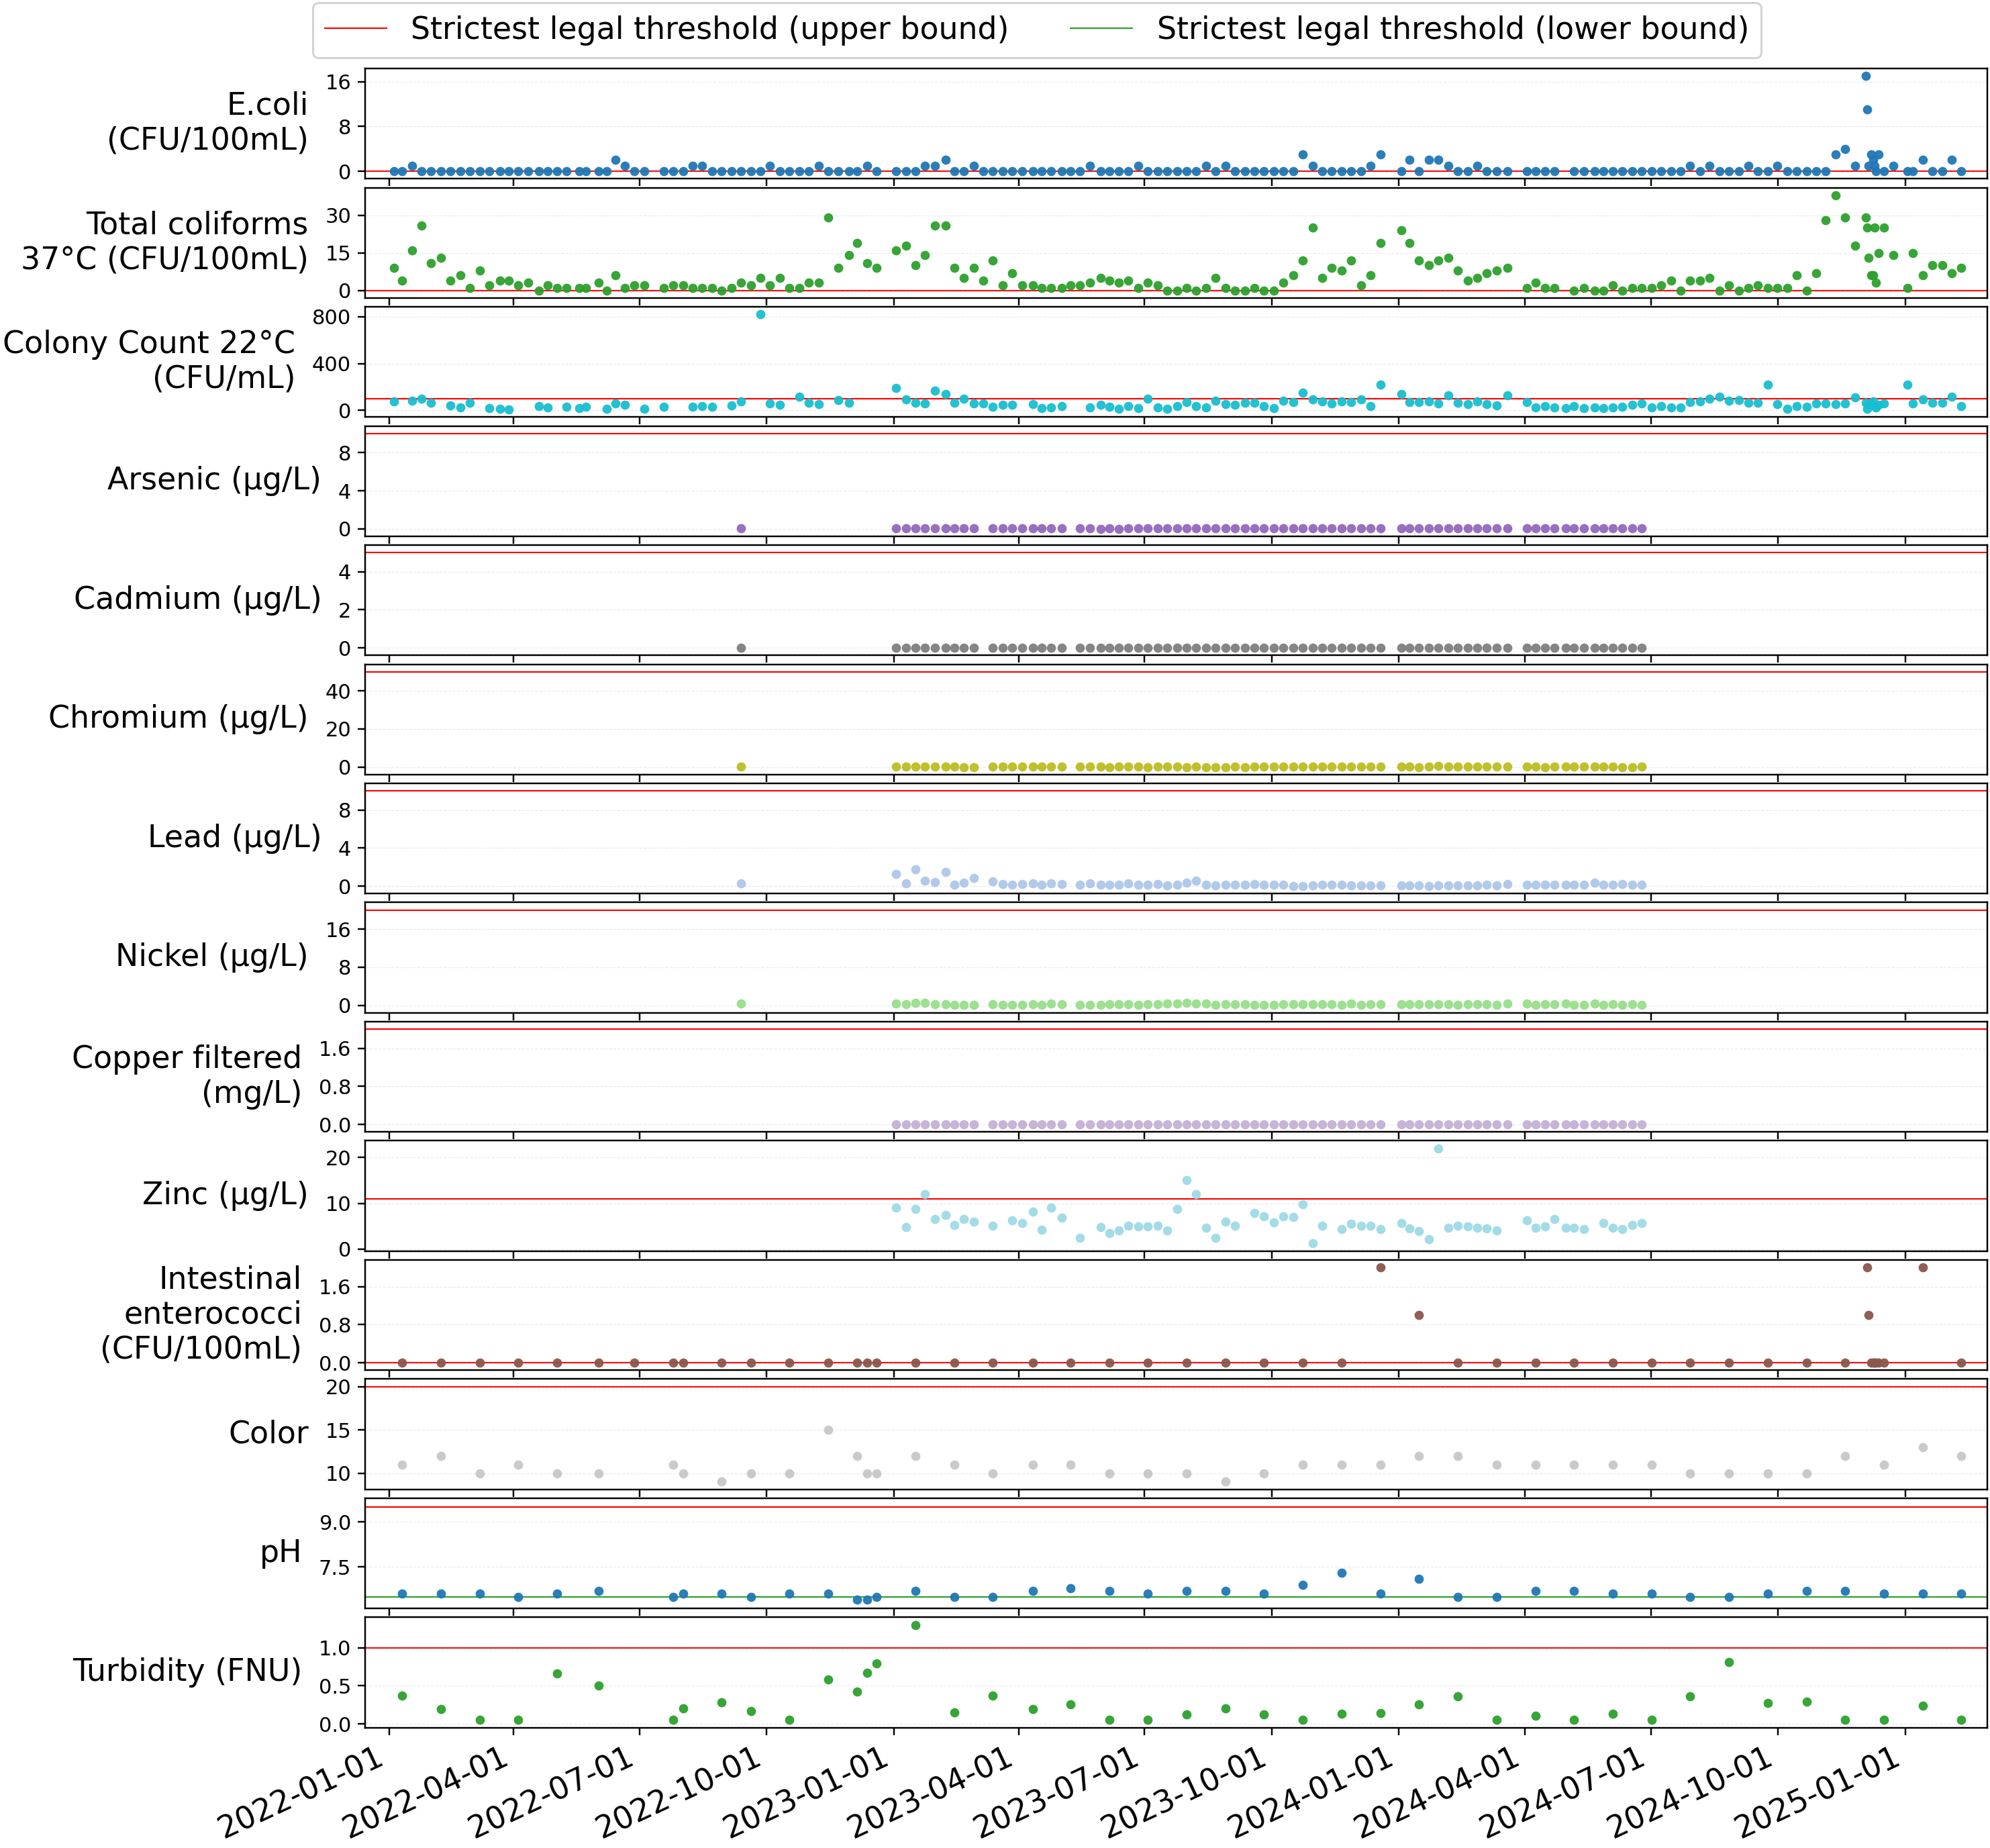
\includegraphics[width=1\linewidth]{figures/Target_timeseries_no_raster.png}
    \caption{Selected water quality parameters from monitoring in the study area.}
    \label{fig:raw_targets}
\end{figure}

From a data engineering perspective, the problem of forecasting specific water quality parameters combines several challenges. The dimensions of the predictor data collected between each measurement of the target parameters is large, but the number of samples 

There is extensive research into automating detection methods for hazardous substances and organisms. (Present several examples and review papers) However, to date these methods have not been commercialized to such an extent that they are accessible within the operational constraints of water utility operators or regulators. There is therefore continued interest in "virtual" or "soft" sensing methods, which assess the presence. There has been extensive research into virtual sensors for environmental water quality. Much of this research has focused not on 


\citep{Wu2020} used data-driven machine learning methods to show that correlations within sampling data can be used infer concentrations  from physical parameters which are quicker to assess. However, this dataset does not address spatial distributions, as all measurements and predictions represent the same physical location.* Also review forecast horizon here. May provide some non-negligible horizon, or not.

Liu et al. \citep{Liu2024} showed that data-driven machine learning analysis of online sensor data can be used to identify anomalous water quality sensor readings, using a subset of one of the same datasets used in this study. However, the interpretation and appropriate response to such anomalies is unclear. The methods' use may be limited to identifying measurement error in sensors. Operationally, more analysis would be needed to determine how to mitigate harm using this method.

Xia et al. \citep{Xia2022} and Feldbauer et al. \citep{Field2007} are recent examples show that process-based models can provide accurate forecasting of some water quality parameters in lakes. 

Xu et al. \citep{Xu2024} is one example establishing that data-driven methods can provide accurate water quality forecasts. But, when flow direction is not constant, sensor placement is non-trivial. There is no clear hierarchy of "upstream" and "downstream" points. 

%Other ideas to touch on: why are sensors not able to automate contaminant detection; why is treatment not robust to any and all contaminants; what natural and anthropogenic hazards make detecting changes to water quality worth accelerating via automation.

This study investigates the extent to which multivariate, data‑driven modeling approaches using time‑series data from in‑situ water quality sensors and local meteorological observations improve the forecasting of trace‑level concentrations of hazardous substances, microbial pathogens, and physicochemical conditions in lentic waters, relative to univariate techniques.

The relative contribution of each water quality indicator and meteorological variable to predictive performance in estimating trace concentrations of hazardous substances, pathogens, and related lentic‑water conditions within data‑driven modeling frameworks?

What forecasting horizons can data‑driven modeling approaches reliably achieve when predicting trace concentrations of hazardous substances, pathogens, and related water‑quality conditions in lentic systems using high‑frequency sensor and meteorological time‑series inputs?


%Make sure to establish context broadly enough to influence Fjordlab: find examples discussing complexity of spatial distribution when flow is 

%%%%%%%%%%%%%%%%%%%%%%%%%%%%%%%%%%%%%%%%%%
\section{Materials and Methods}
\label{ch:MaterialsMethods}

% \subsection{Structure}
% \label{ch:Structure}

The study compares the performance of several common machine learning algorithms on a series of regression tasks for predicting water quality in a lake. The models are configured to predict parameters which are immediate safety hazards, rather , providing improved specificity compared to indicator  Performance is quantified in terms o

\begin{enumerate}
    \item Which parameters can 
\end{enumerate}

\subsection{Study Area}
\label{ch:StudyArea}
The subject of the study is Brusdalsvatnet, a glacial lake in Ålesund, Norway pictured in Fig.~\ref{fig:map}. As the principle or secondary raw water source for public water supplies serving a combined population of approximately 70,000, raw water quality at the intake for a treatment plant is regularly sampled, analyzed and reported per Norwegian law. Water is abstracted from an offtake located at a depth of approximately 35 m and pumped to a treatment plant at Vasstrandlia, where raw water samples and measurements are collected. An assessment of the tributary network derived from a digital elevation model illustrates the topological problem whereby many parallel inflows from comparable catchment areas enter the lake.

\begin{figure}
    \centering
    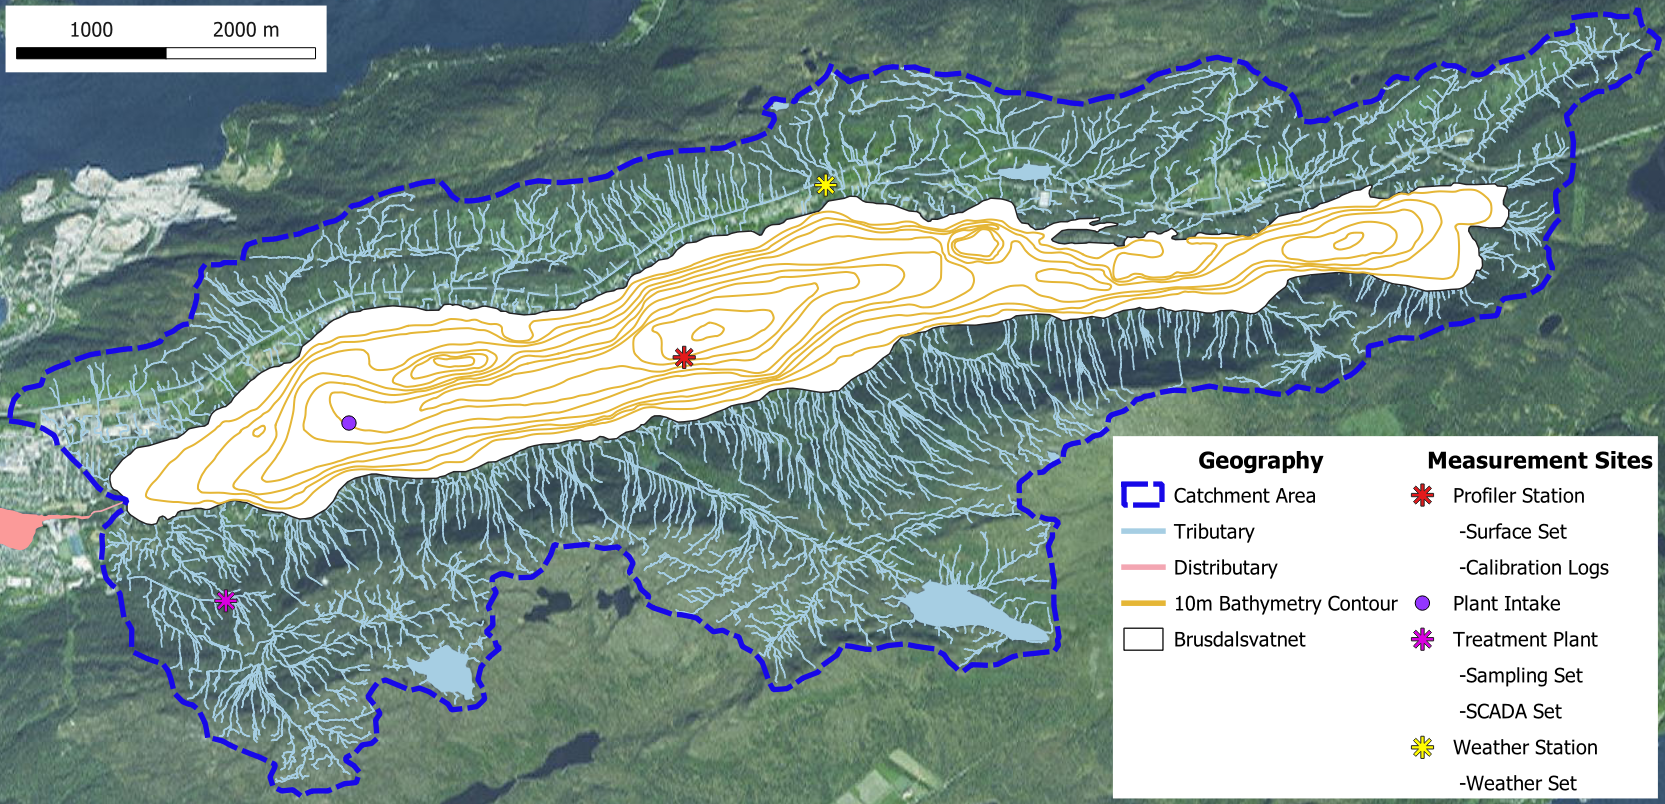
\includegraphics[width=1\linewidth]{figures/map.png}
    \caption{Brusdalsvatnet hydrological features.}
    \label{fig:map}
\end{figure}

In line with WHO guidelines and local law,  a minimum set of parameters and monitoring frequencies for drinking water surface sources. Additional monitoring can be required to address specific hazards identified by risk assessments. Hazards present in the Brusdalsvatnet these hazards include sewage overflows from both municipal and individual wastewater systems, highway-related emissions such as soot and tire and road wear particles, and other industrial activity in the watershed such as construction.

\subsection{Datasets}
\label{ch:Datasets}
The study uses a time series dataset spanning from 3 January 2022 to 10 February 2025 which combines a total of 31 features aggregated from five independent sources. An additional dataset of calibration records for one of the sources is used to estimate measurement error for those features. The mixed frequency, mixed coverage, mixed scales, noise, and measurement error present in the dataset make the use of conventional regression methods challenging. All values for all features are normalized onto the interval [0,1]. For each target, samples are split using a 70/30 temporal train/test split based on total data (count of predictor and target measurements), to prevent future data leaking into training while ensuring adequate data for fair evaluation. 

The target features in the set \textbf{Samples} represent the ground truth for concentrations of hazardous substances and pathogens. Rather than target the measured values, the models are trained and evaluated on the differential from the previous measurement. as shown in Fig.~\ref{fig:targets}, along with a raster bar depicting variation in the availability of the 17 predictor features. The values are determined by laboratory analysis of raw water samples taken during normal operation from influent to the Vasstrandlia water treatment plant, after being pumped from the offtake up to the plant. No information is available describing the uncertainty in these measurements.

\begin{figure}
    \centering
    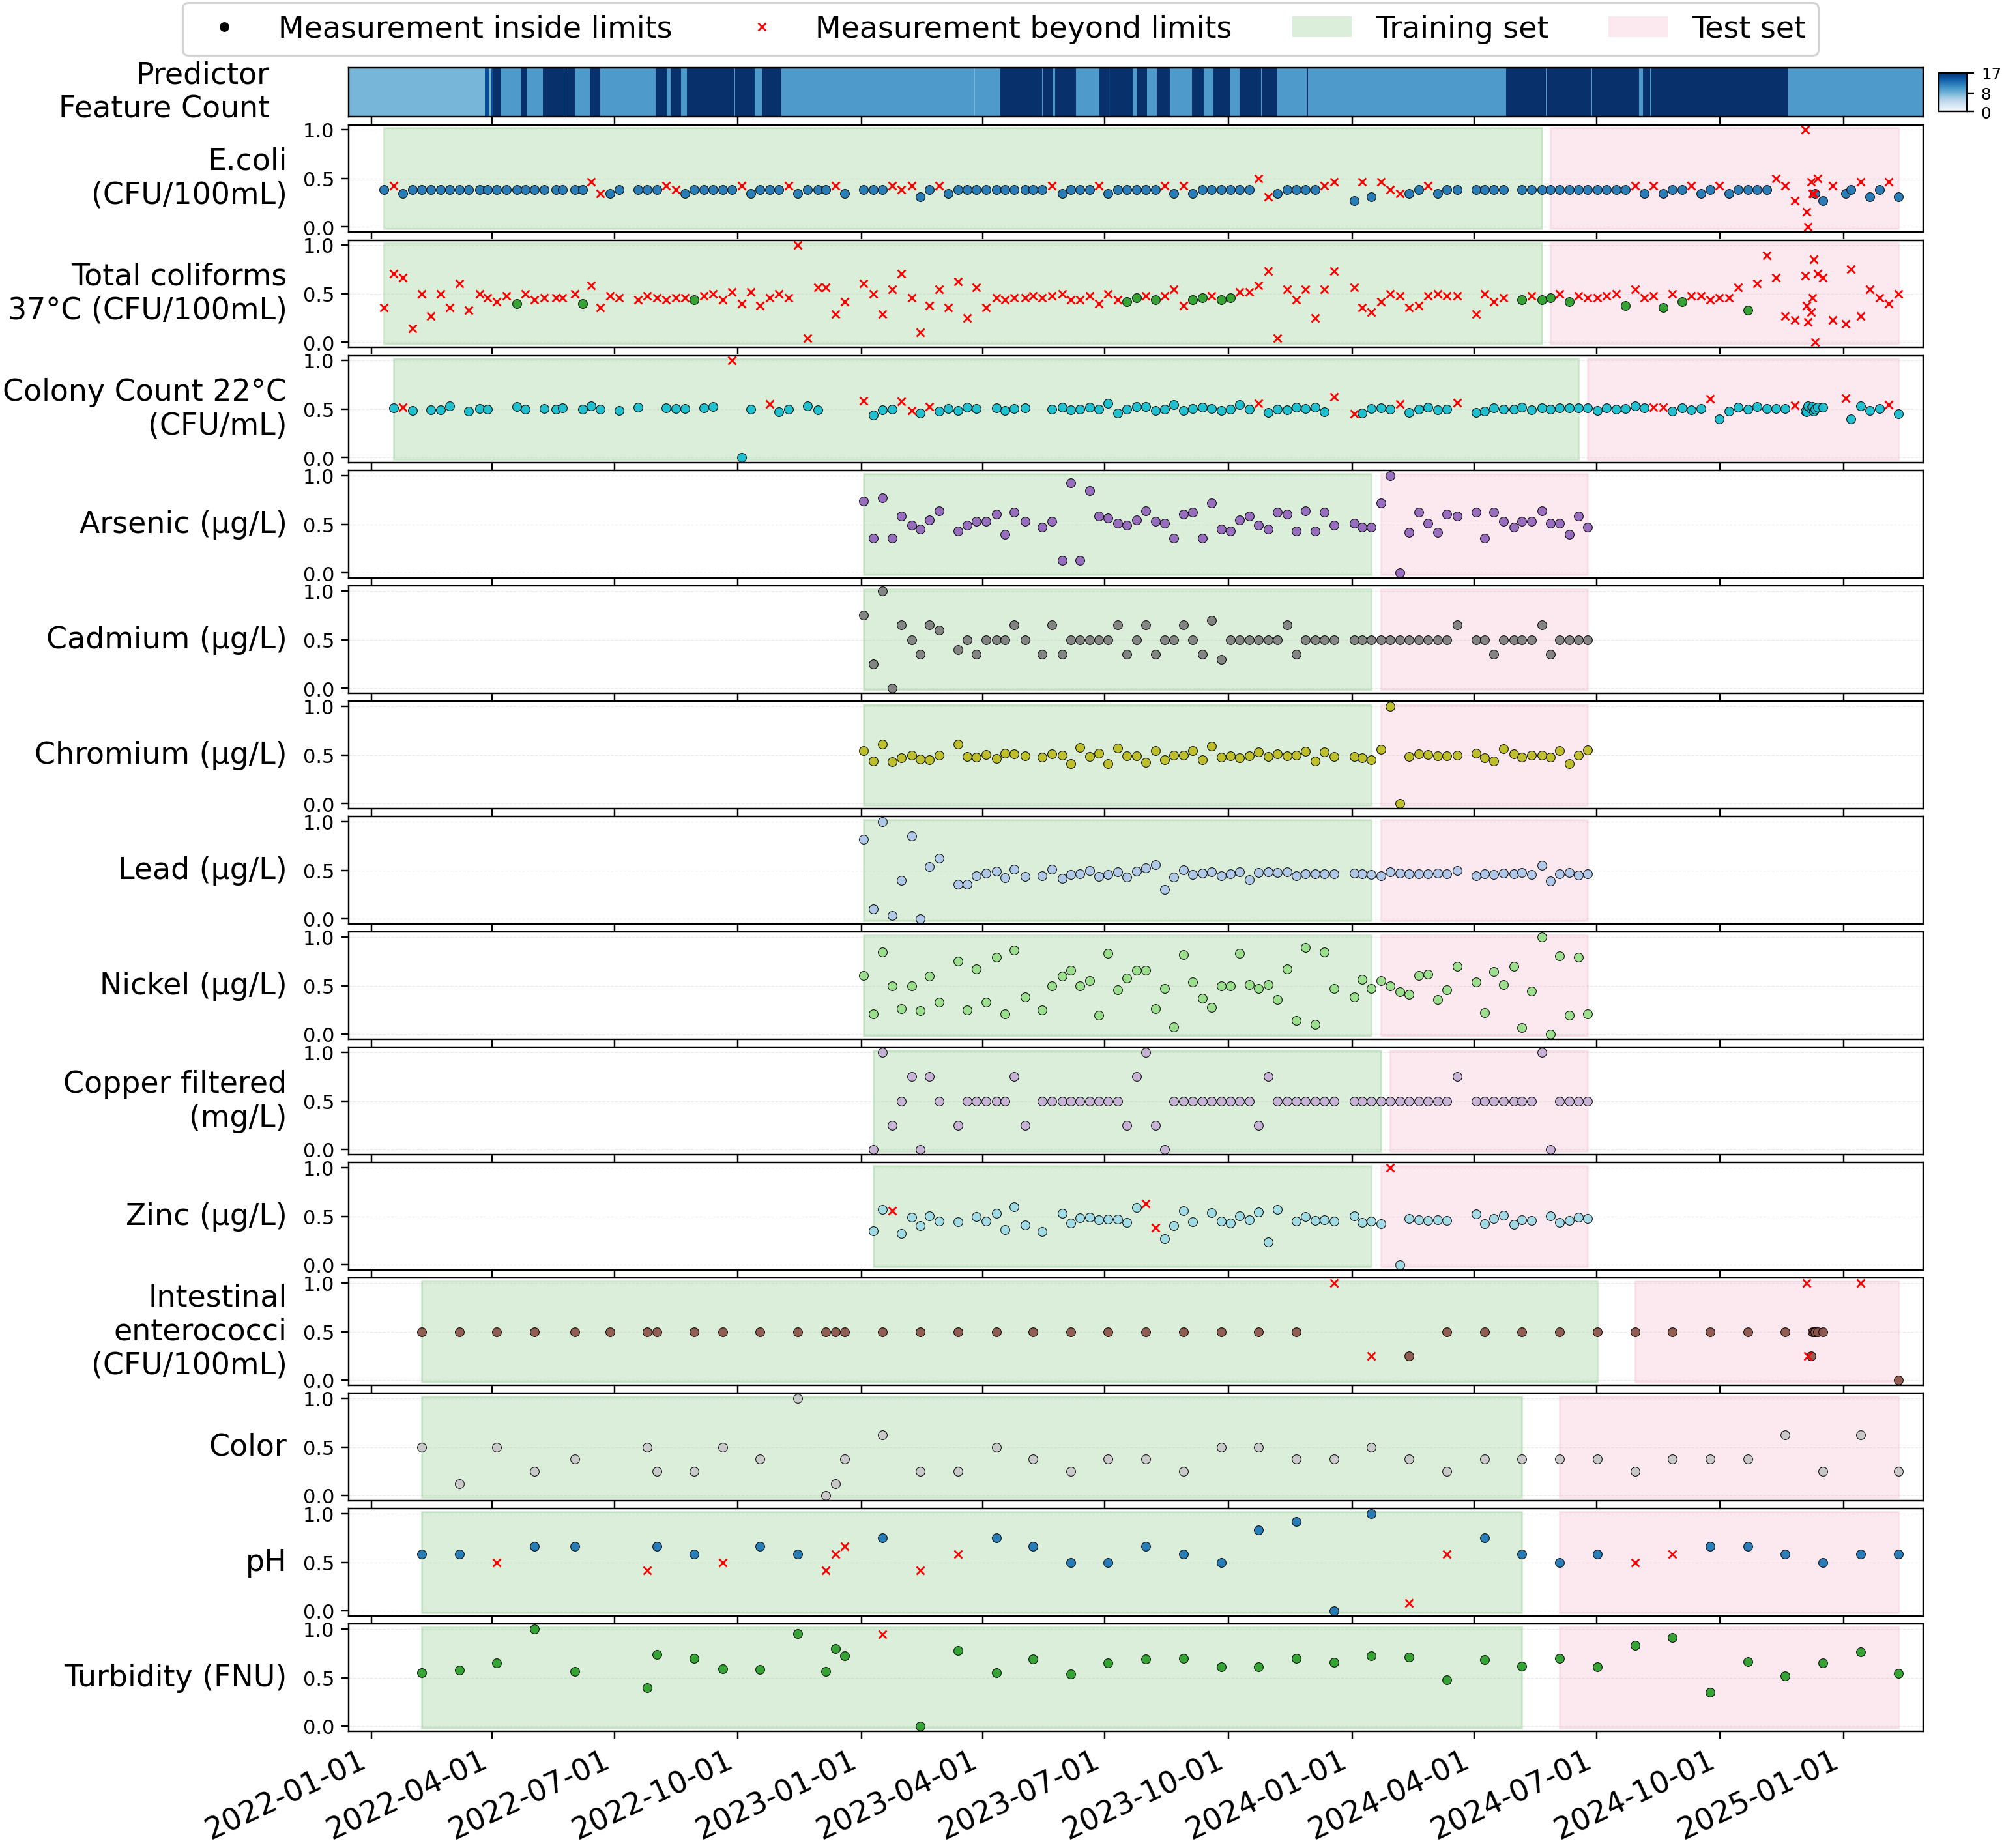
\includegraphics[width=1\linewidth]{figures/Target_diff_timeseries_overlay_norm.png}
    \caption{Samples dataset: train-test split of normalized change in hazardous substance concentrations.}
    \label{fig:targets}
\end{figure}

The \textbf{Surface} set plotted in Fig.~\ref{fig:surface} consists of hourly automated reading from an EXO sonde by YSI Integrated Services \& Systems, deployed from the Vertical Profiler System by YSI at a fixed depth of approximately 2.3m. This set has the most limited coverage, as the platform is sensitive to disturbances and cannot be operated during winter months due to icing. Sensors were regularly re-calibrated in accordance with manufacturer recommendations, yielding the additional dataset \textbf{Calibrations} used to estimate the per-sensor distributions of measurement error. In spite of regular calibration and model treatment of measurement error, some measurements are rejected as invalid based on expected physical limits.

\begin{figure}
    \centering
    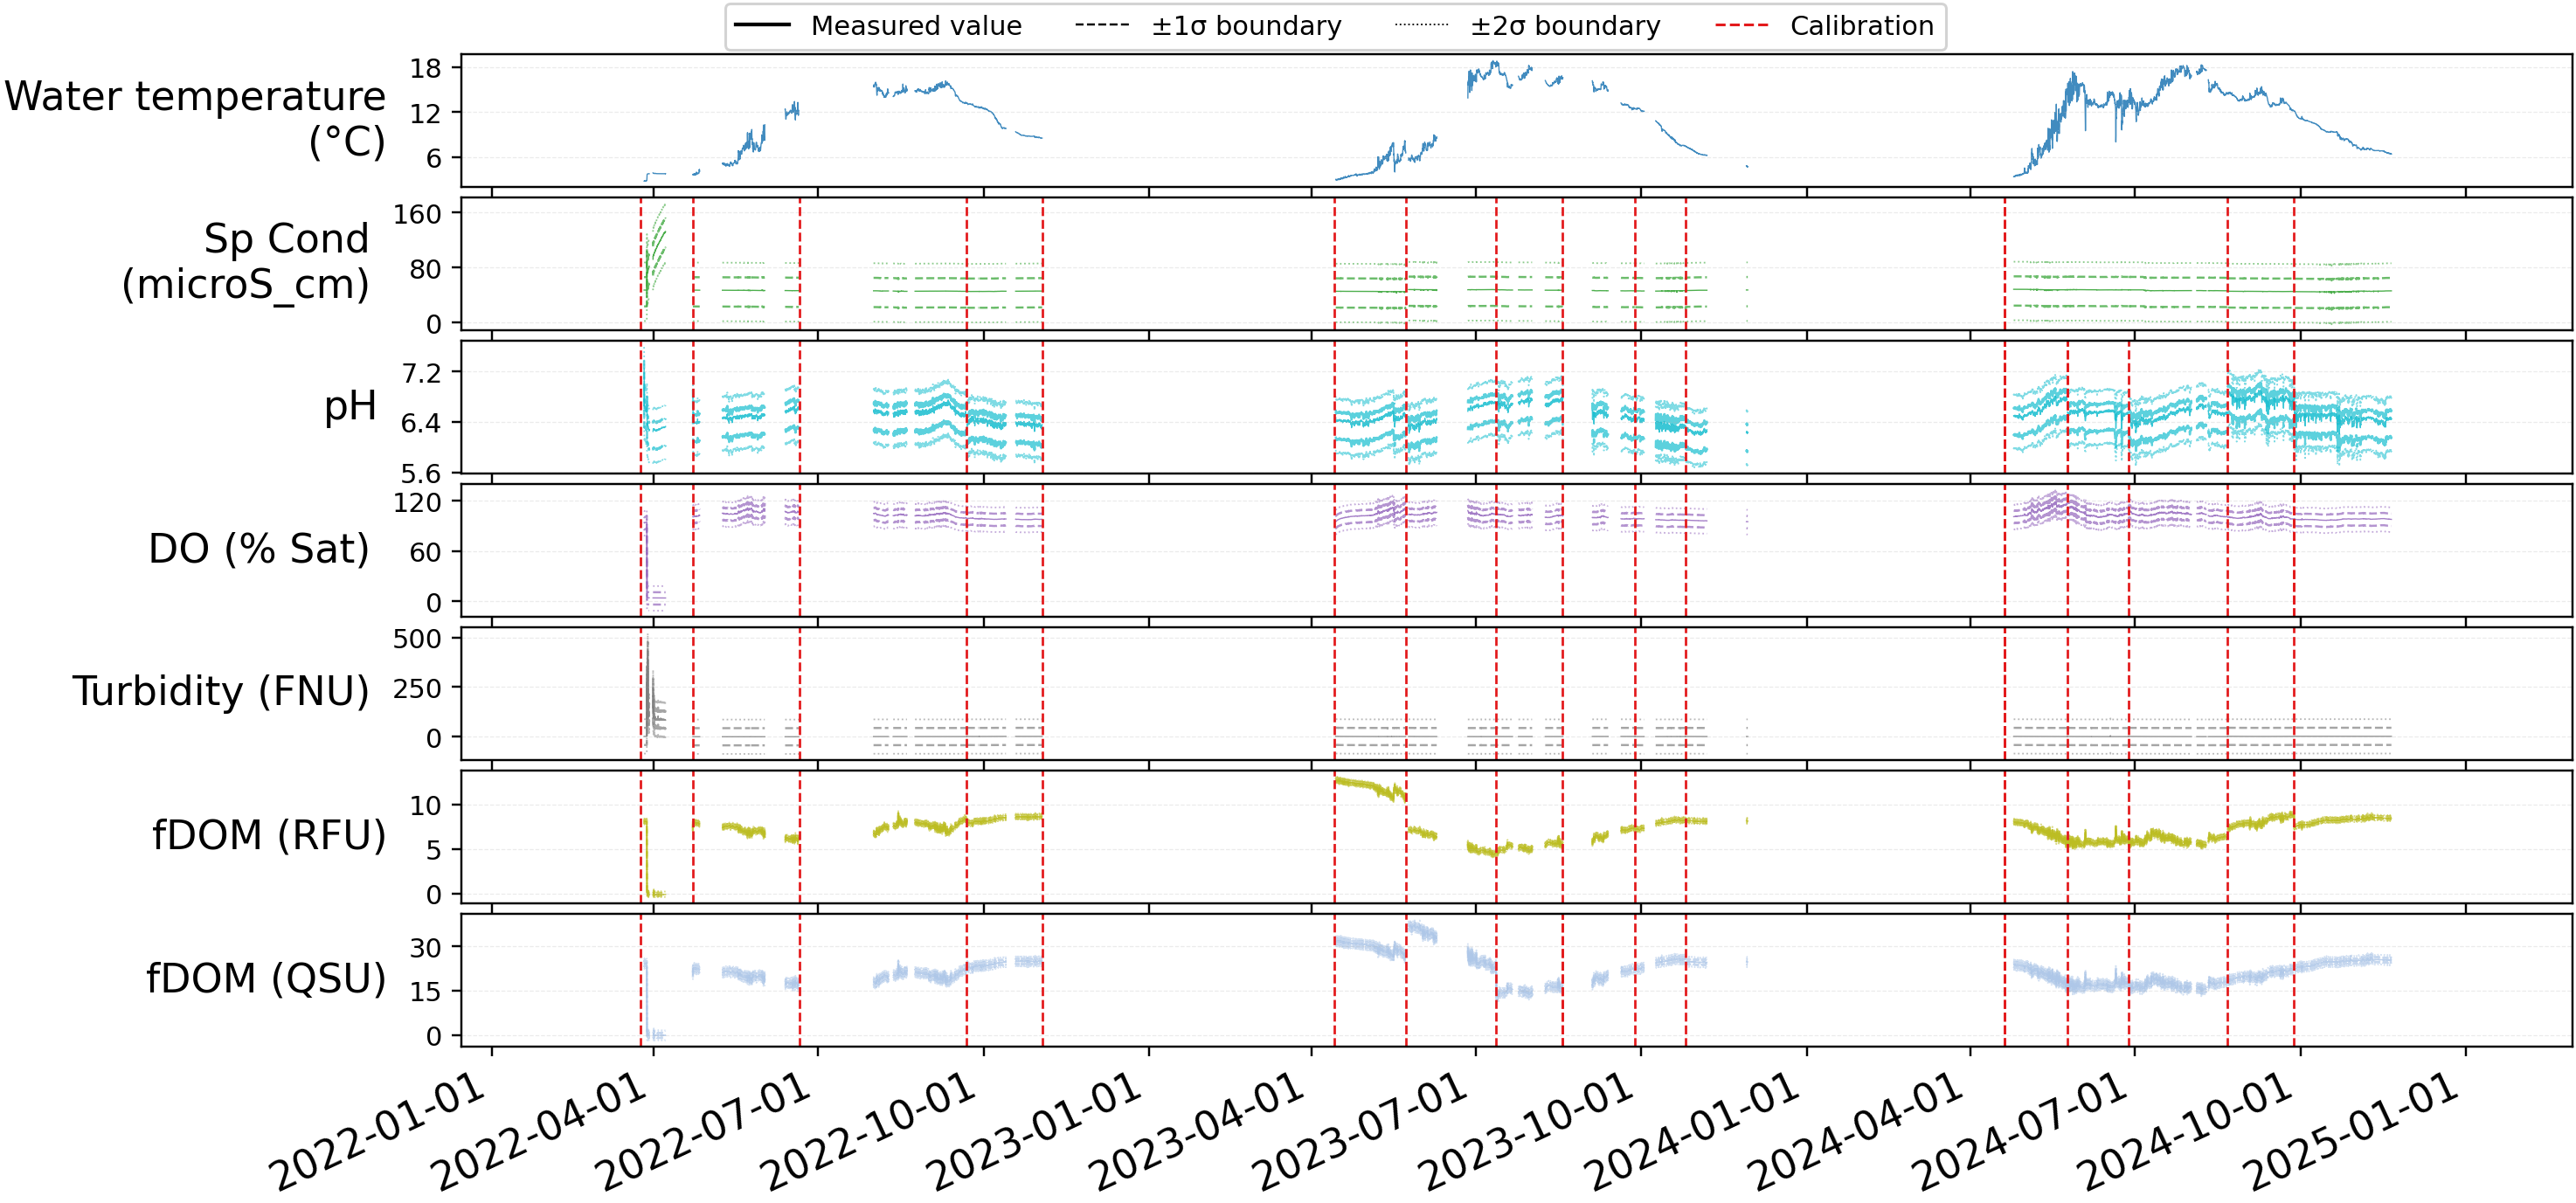
\includegraphics[width=1\linewidth]{figures/Surface_timeseries_uncertainty.png}
    \caption{Surface dataset features with estimated measurement error distributions.}
    \label{fig:surface}
\end{figure}

\textbf{SCADA}: The Vasstrandlia water treatment plant's SCADA system measures limited water quality parameters of the same influent raw water as assessed in Samples at a one minute sample rate. The series are downsampled to hourly frequency by averaging to match the other predictor features, plotted in Fig.~\ref{fig:SCADA}. Note that the pH series exhibits unusual trends which could indicate measurement error or data quality problems, but no calibration data is available to assess.

\begin{figure}
    \centering
    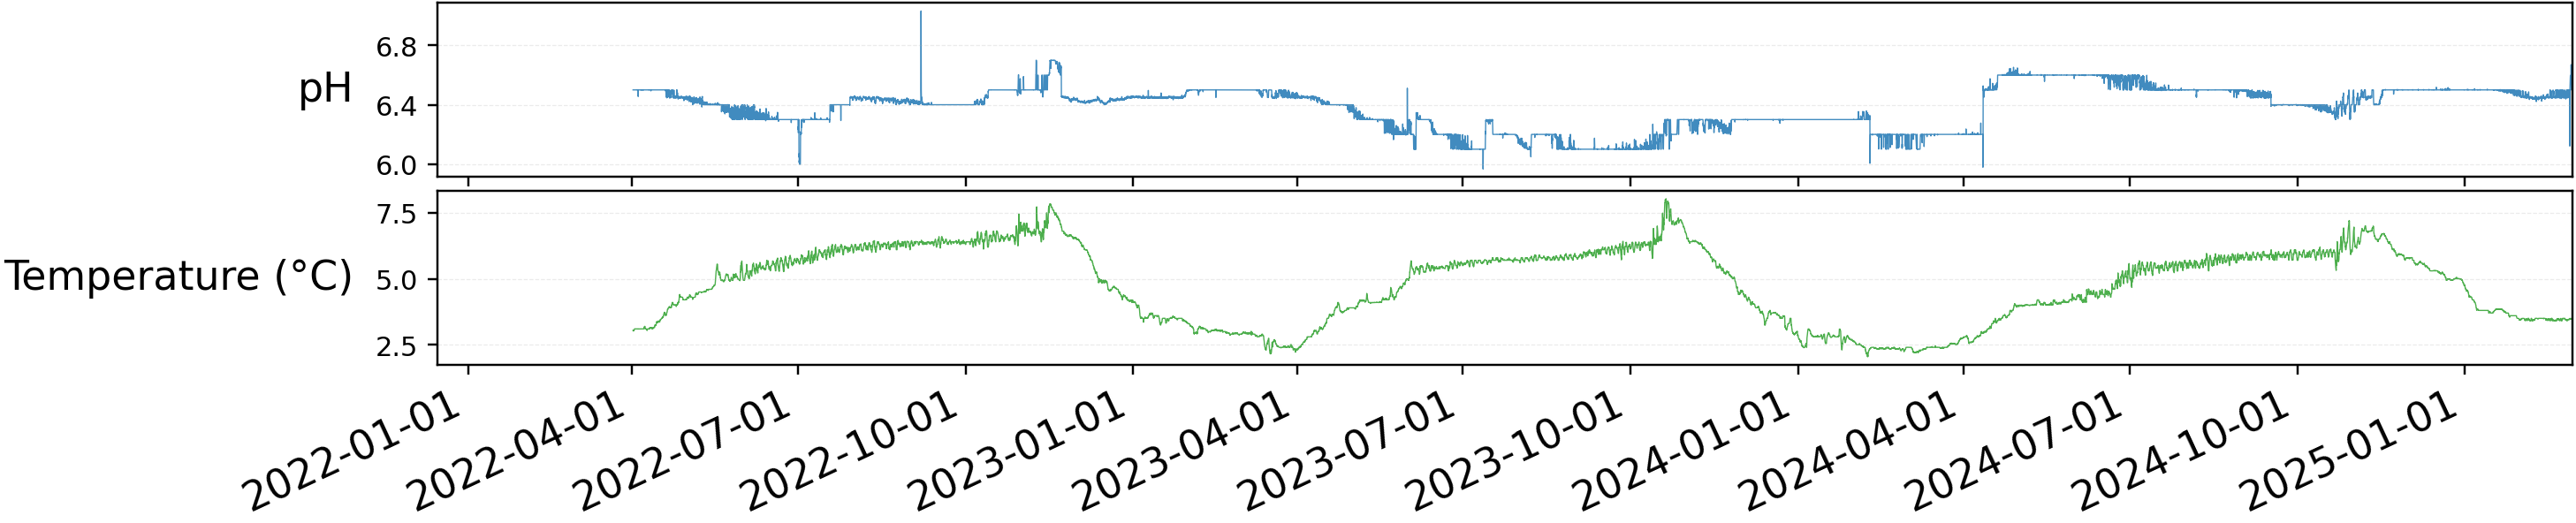
\includegraphics[width=1\linewidth]{figures/SCADA_timeseries.png}
    \caption{SCADA dataset features.}
    \label{fig:SCADA}
\end{figure}

The \textbf{Weather} set shown in Fig.~\ref{fig:weather} is derived from two sources. A station located on land within the watershed provides sensor measurements, but there are gaps in coverage. Missing values are filled with values extracted via API from the Norwegian Meteorological Institute's NORA3 near-surface analysis, a forecast which was retroactively corrected to better match ground truth sensor values collected during the period where the forecast applied. The analysis is specific to the 1 km grid square where the sensor is located, corrected for elevation.

\begin{figure}
    \centering
    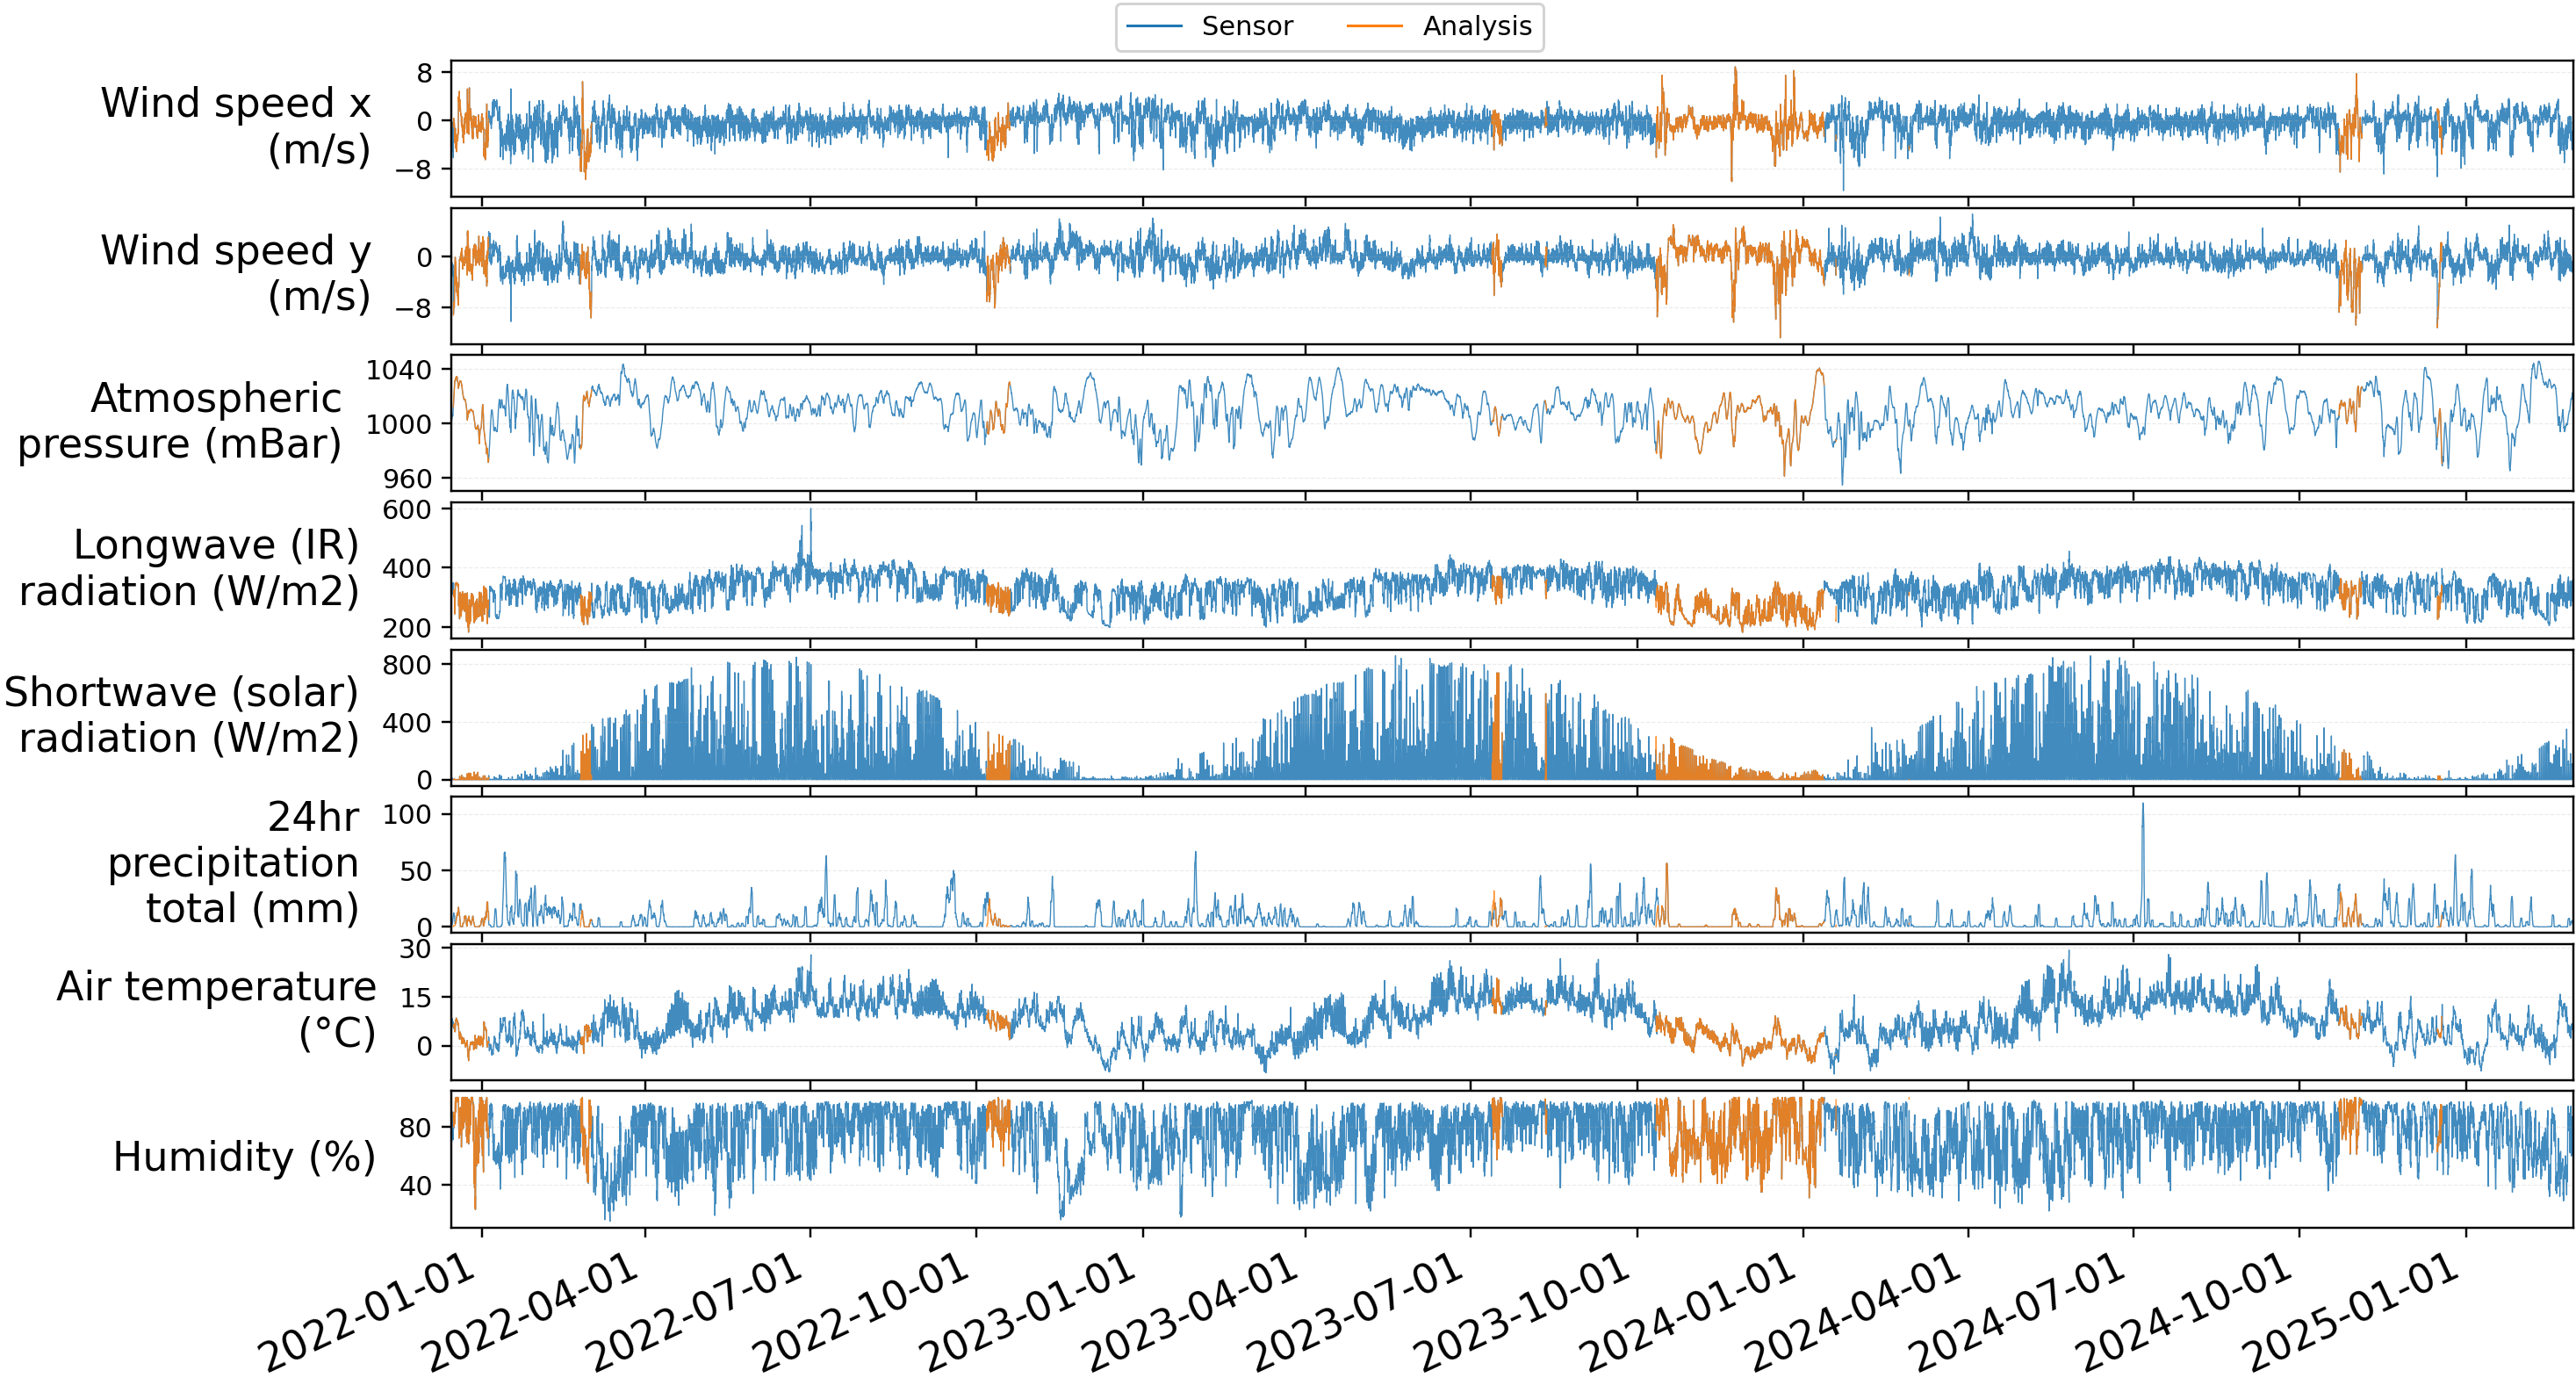
\includegraphics[width=1\linewidth]{figures/Weather_timeseries_alt_source.png}
    \caption{Weather features, by source.}
    \label{fig:weather}
\end{figure}


\subsection{Forecasting Methods}
\label{ch:ForecastingMethods}
For each target parameter, models were trained and evaluated using four supervised learning machine learning methods. Each model uses training samples consisting of fixed-length windows of predictor sensor measurements based on the median sampling interval, which is consistennt  (e.g. 168 hourly rows × $d$ sensor columns). The regression target is a scalar from the final row of that window.  Let $\mathbf{X} \in \mathbb{R}^{T \times d}$ be the input window and $y \in \mathbb{R}$ the target. 

\textbf{XGBoost} "Extreme gradient boosting" is a decision-tree based algorithm introduced in \citep{Chen2016} and implemented in the open source Python library XGBoost. An advantage of the XGBoost method is that it is tolerant of missing predictor values, which means that fewer of the limited number of valid targets are eliminated from the training and testing sets because of missing data. 

\textbf{Transformer} Transformers are a type of artificial neural network which use 'attention' to weight feature importance during the forward training loop. The structure is . However, it is sensitive to missing values, which can limit the number of samples available for training and testing the model when  The model is implemented using the PyTorch Python library introduced in /cite{Paszke2019}.

A \textbf{Gaussian Process} (GP) model is based on the assumption that any set of function values has a joint multivariate Gaussian distribution, represented using a mean function and a kernel function chosen to represent the covariance between each pair of points in the dataset.  Given training data $\mathcal{D} = \{(\mathbf{x}_i, y_i)\}_{i=1}^{n}$, the predictive posterior at
a new point $\mathbf{x}_*$ is: 
$$p(y_* \mid \mathbf{x}_*, \mathcal{D}) = \mathcal{N}(\mu_*, \sigma_*^2)$$ 
$$\mu_* = \mathbf{k}_*^\top (\mathbf{K} + \sigma_n^2 \mathbf{I})^{-1} \mathbf{y}$$ 
$$\sigma_*^2 = k(\mathbf{x}_*, \mathbf{x}_*) - \mathbf{k}_*^\top (\mathbf{K} + \sigma_n^2 \mathbf{I})^{-1} \mathbf{k}_*$$ 

where $\mathbf{K}_{ij} = k(\mathbf{x}_i, \mathbf{x}_j)$ and $\sigma_n^2$ is the observation noise variance.  This model is implemented using the GPyTorch Python package introduced in \cite{Gardner2018}. 

The selected kernel is `matern52+linear`, composed as: $$k(\mathbf{x}, \mathbf{x}') = \sigma_f^2\, k_{\text{Matérn52}}(\mathbf{x}, \mathbf{x}') + k_{\text{linear}}(\mathbf{x}, \mathbf{x}')$$ where $\sigma_f^2$ is an output scale with a $\text{Gamma}(2.0, 0.15)$ prior.

$$k_{\text{Matérn52}}(\mathbf{x}, \mathbf{x}') = \left(1 + \sqrt{5}\,r + \frac{5}{3}r^2\right) e^{-\sqrt{5}\,r}$$

where $r = \sqrt{(\mathbf{x}-\mathbf{x}')^\top \boldsymbol{\Lambda}^{-2} (\mathbf{x}-\mathbf{x}')}$
and $\boldsymbol{\Lambda} = \text{diag}(\ell_1, \ldots, \ell_d)$ is the ARD
lengthscale matrix.

The per-sensor variance $\sigma_j^2$ is derived from aggregate calibration offsets fitted to a Student's $t$ distribution. 

The linear additive term captures any long-run monotone trends (e.g. gradual sensor drift between calibrations) that stationary kernels alone cannot represent. 

Thus GP models handle uncertainty distributions for predictor parameters and target predictions explicitly, avoiding the Monte Carlo replicates used in training and evaluating of the other ML model types.

For each forecasted target, a dimensionally equivalent prediction is also computed using three simple non-machine learning algorithms to provide a baseline for comparison. 

The \textbf{Na\"ive} model (also known as the persistence or a forward fill) models each target as constant at the most recently measured value.   $$\hat{y}(t) = y(t^{*}), \quad t^{*} = \max\{t_k : t_k \leq t_c,\; y(t_k) \text{ is valid}\}$$


\textbf{Linear} Linearly extrapolate the target value using all target values, to reflect the trend of a defined window.

\textbf{Seasonal} Given the strong seasonality of environmental processes at the high latitude of the study area, including diurnal and annual trends, this method averages values from other samples taken at similar phases. Due to the limited extent of the Sampling dataset, data leakage is permitted in this model: averages are taken across all years in the dataset except the year of the prediction, including future years. The seasonal baseline predicts each forecast time step as the mean of historically observed values at similar times of year and time of day, excluding the current year to prevent data leakage. Similarity is determined by a hierarchical windowing strategy that relaxes constraints until a sufficient sample ($\geq 3$ values) is found. For a forecast at day-of-year $d$ and hour-of-day $h$, the prediction is computed from prior-year observations using the first matching tier: $$\hat{y}(d, h) = \frac{1}{|\mathcal{W}|}\sum_{i \in \mathcal{W}} y_i$$

where $\mathcal{W}$ is the set of valid historical values matching the narrowest sufficient window tier:

| Tier | Day-of-year constraint | Hour-of-day constraint |
|------|----------------------|----------------------|
| 1 | $|d_i - d| \leq W_{\text{day,narrow}}$ (circular) | $|h_i - h| \leq W_{\text{diurnal}}$ |
| 2 | $|d_i - d| \leq W_{\text{day,narrow}}$ (circular) | none |
| 3 | $|d_i - d| \leq W_{\text{day,wide}}$ (circular) | none |
| 4 | all prior-year values | none |


\subsection{Modeling Pipeline}
\label{ch:ModelingPipeline}

Models for forecasting each target are developed and evaluated independently using the process illustrated in Fig.~\ref{fig:pipeline}. For each target, the process searches for the feature set and model type which provide the most accurate predictions at the specified forecast horizon, while implementing robust regularization to compensate for the small sample sizes in both the training and test sets. With so much predictor data per target and sufficient iterations, inadequately regularized methods can find predictive trends even in completely unrelated data. With 18 predictor parameters, there are $2^{18}$ possible feature combinations, so a global search method is infeasible. Instead, the model uses a two-stage directed . This method is not guaranteed to find the best possible feature set.


The experiments were conducted in the computing environment described in Table~\ref{tab:computer}.

\begin{table}[H] 
%\small % Change table font size
\caption{Computing Environment\label{tab:computer}}
%\isPreprints{\centering}{} % Only used for preprints
\begin{tabularx}{\textwidth}{CC}
\toprule
\textbf{Component}	& \textbf{Specification}\\
\midrule
CPU		& Intel Core i7-14700 (2.10 GHz)\\
Memory		& 32 GB RAM\\
GPU		& NVIDIA GeForce RTX 4070 12 GB\\
Operating System		& Windows 11 Pro\\
\bottomrule
\end{tabularx}
\end{table}

\begin{itemize}
    \item \textbf{Surrogate-guided beam search with backward elimination and optional swap refinement} is applied as a robust feature selection method, to identify the subset of available predictor variables which provides the most accurate predictions for 
    \item \textbf{Rolling origin cross validation (LOOCV)} Like k-fold cross validation, this provides a measure of how well a model will generalize to new data by evaluating the sensitivity of prediction accuracy to the split of samples into training and test sets. Because of the strict time-based split necessary to prevent data leakage in time series datasets, this is the best available common cross validation method.
    \item 
\end{itemize}

\subsection{Evaluation Metrics}
The forecasting ability of the best ML model found for each target is evaluated in terms of the accuracy compared to the ground truth values in the evaluation set; skill relative to the baseline models; and the statistical significance of the forecast skill, given the characteristics of the evaluation set. Forecast accuracy relative to the ground truth is measured using simple descriptive statistics including mean absolute error (MAE), root mean square error (RMSE), Pearson correlation coefficient (r), and the coefficient of determination (R\textsuperscript{2}). Forecast skill score (SS) is derived from the ratio of RMSE in the most-accurate baseline model and the ML model, as shown in Eq. \ref{eq:skill}.

\begin{equation} \label{eq:skill}
    \text{SS} = \min_{b \in {baselines}} 1 - \frac{\text{RMSE}_{\text{model}}}{\text{RMSE}_b}
\end{equation}

Assessing the statistical significance of the forecast skill requires more complex tests, summarized in \ref{tab:stats}. 

\begin{table}[H] 
%\small % Change table font size
\caption{Reliability Tests\label{tab:stats}}
%\isPreprints{\centering}{} % Only used for preprints
\renewcommand{\arraystretch}{1.4}
\begin{tabularx}{\textwidth}{
    >{\hsize=0.8\hsize\raggedleft\arraybackslash}X 
    >{\hsize=1\hsize\raggedright\arraybackslash}X
}
\toprule
\textbf{Test} & \textbf{Condition}\\
\midrule
Bootstrap Lower Confidence Bound & $\text{LCB}_{95\%}^{(b)} > 0$ \\
Diebold-Mariano & $p_{\text{DM}} < \alpha$ and $\text{DM} < 0$ \\
Wilcoxon & $p_{\text{Wilcoxon}} < \alpha$ \\
Sign Test & $p_{\text{Sign}} < \alpha$ and Win Rate $> 0.5$ \\
Coverage & deficit $\leq \tau$ and deficit $\leq$ baseline deficit $+ \tau$

\end{tabularx}
\end{table}

An aggregate "Evidence Score" is calculated to categorize the trustworthiness of each model, calculated as the number of statistical tests where the forecast passed the test 

$$S_b = G_{\text{lcb}}^{(b)} + G_{\text{dm}}^{(b)} + G_{\text{wilc}}^{(b)} + G_{\text{sign}}^{(b)} + G_{\text{cov}}^{(b)} \quad \in \{0, 1, 2, 3, 4, 5\}$$

$$S_{\text{overall}} = \min_{b \in \{baselines} \Sigma $$



Diebold-Mariano (DM) Test
Compares forecast accuracy between two models:
$$
DM = \frac{\bar{d}}{\sqrt{\frac{\hat{\gamma}_d(0) + 2 \sum_{k=1}^{h-1} \hat{\gamma}_d(k)}{n}}}
$$
Where:
- $\bar{d}$: mean difference in loss (e.g., RMSE) between models; $\hat{\gamma}_d(k)$ is autocovariance at lag $k$; and $n$ is the number of samples

2. Wilcoxon Signed-Rank Test
Non-parametric test for paired differences:
- Compute signed ranks of differences $d_i$ (excluding zeros).
- Test statistic $W$ is the sum of ranks for positive differences.

3. Sign Test
Counts wins/losses:
$$
n_{win} = \sum_i \mathbb{I}(d_i < 0) \qquad n_{loss} = \sum_i \mathbb{I}(d_i > 0)
$$
$p$-value from binomial test under $H_0: p=0.5$.

4. Cohen's d (Effect Size)
$$
d = \frac{\bar{d}}{s_d}
$$
Where $\bar{d}$ is the mean of differences, $s_d$ is their standard deviation.

5. Bootstrap Confidence Intervals
- Resample groups with replacement, recompute skill metric (e.g., $1 - \frac{\text{RMSE}_\text{model}}{\text{RMSE}_\text{baseline}}$).
- Compute percentiles for confidence intervals.

6. ANOVA Variance Components
Decompose variance into within-group and between-group components. Intra-class correlation coefficient (ICC):
$$
\text{ICC} = \frac{\text{MS}_{\text{between}}}{\text{MS}_{\text{between}} + \text{MS}_{\text{within}}}
$$

The Evidence Score is a summary metric (e.g., mean skill improvement, probability model outperforms baseline) computed across independent test groups. Statistical tests (DM, Wilcoxon, Sign) are applied to the distribution of per-group differences in error or skill between model and baseline. Bootstrap is used to estimate confidence intervals and the probability that the model outperforms the baseline ($P(\text{skill} > 0)$). Cohen's d quantifies the effect size of the improvement. ANOVA may be used to estimate the fraction of variance attributable to group differences, in this case for uncertainty quantification.


To evaluate the forecast horizon, the lookahead interval at which a model's prediction are not better than a simple baseline, the best-performing model as determined by the process in Ch.~\ref{ch:ModelingPipeline} 

The forecast horizon for each model is quantified in terms of the time over which the forecast $R^2$ decreases to the higher of 0 or the $R^2$ fo the best performing baseline, based on the average rate of decrease observed over horizons increasing from from 1 to 168 hours. Thus if $(h_i, r_i)$ are the horizon points:

\[\label{eq:r2rate}
m_{R^2}
=
\frac{\sum_i (h_i-\bar h)(r_i-\bar r)}{\sum_i (h_i-\bar h)^2}
\]

\[
t_{\text{hours}}=\frac{R^2_{\text{target}}-R^2_{\text{init}}}{m_{R^2}}
\qquad
\]



% Materials and Methods should be described with sufficient details to allow others to replicate and build on published results. Please note that publication of your manuscript implicates that you must make all materials, data, computer code, and protocols associated with the publication available to readers. Please disclose at the submission stage any restrictions on the availability of materials or information. New methods and protocols should be described in detail while well-established methods can be briefly described and appropriately cited.

% Research manuscripts reporting large datasets that are deposited in a publicly avail-able database should specify where the data have been deposited and provide the relevant accession numbers. If the accession numbers have not yet been obtained at the time of submission, please state that they will be provided during review. They must be provided prior to publication.

% Interventionary studies involving animals or humans, and other studies require ethical approval must list the authority that provided approval and the corresponding ethical approval code.

% In this section, where applicable, authors are required to disclose details of how gen-erative artificial intelligence (GenAI) has been used in this paper (e.g., to generate text, data, or graphics, or to assist in study design, data collection, analysis, or interpretation). The use of GenAI for superficial text editing (e.g., grammar, spelling, punctuation, and formatting) does not need to be declared.


%%%%%%%%%%%%%%%%%%%%%%%%%%%%%%%%%%%%%%%%%%
\section{Results}
\label{ch:Results}

\subsection{Model Structure Selection}

Several structural alternatives for input and output data were evaluated over all targets, as summarized using the R\textsuperscript{2} statistic as shown in Fig.~\ref{fig:structure}. "State in, differential out", which includes the previous measurement value (state) as a predictor and targets the differential in the target at the next measurement, was found to perform best across most targets, especially if the confidence of the predictions is taken into account. This structure was used in all subsequent evaluations. Note that the state may still be dropped from the model in the feature selection process. The structure merely determines whether the state is included as an available predictor. 

\begin{figure}
    \centering
    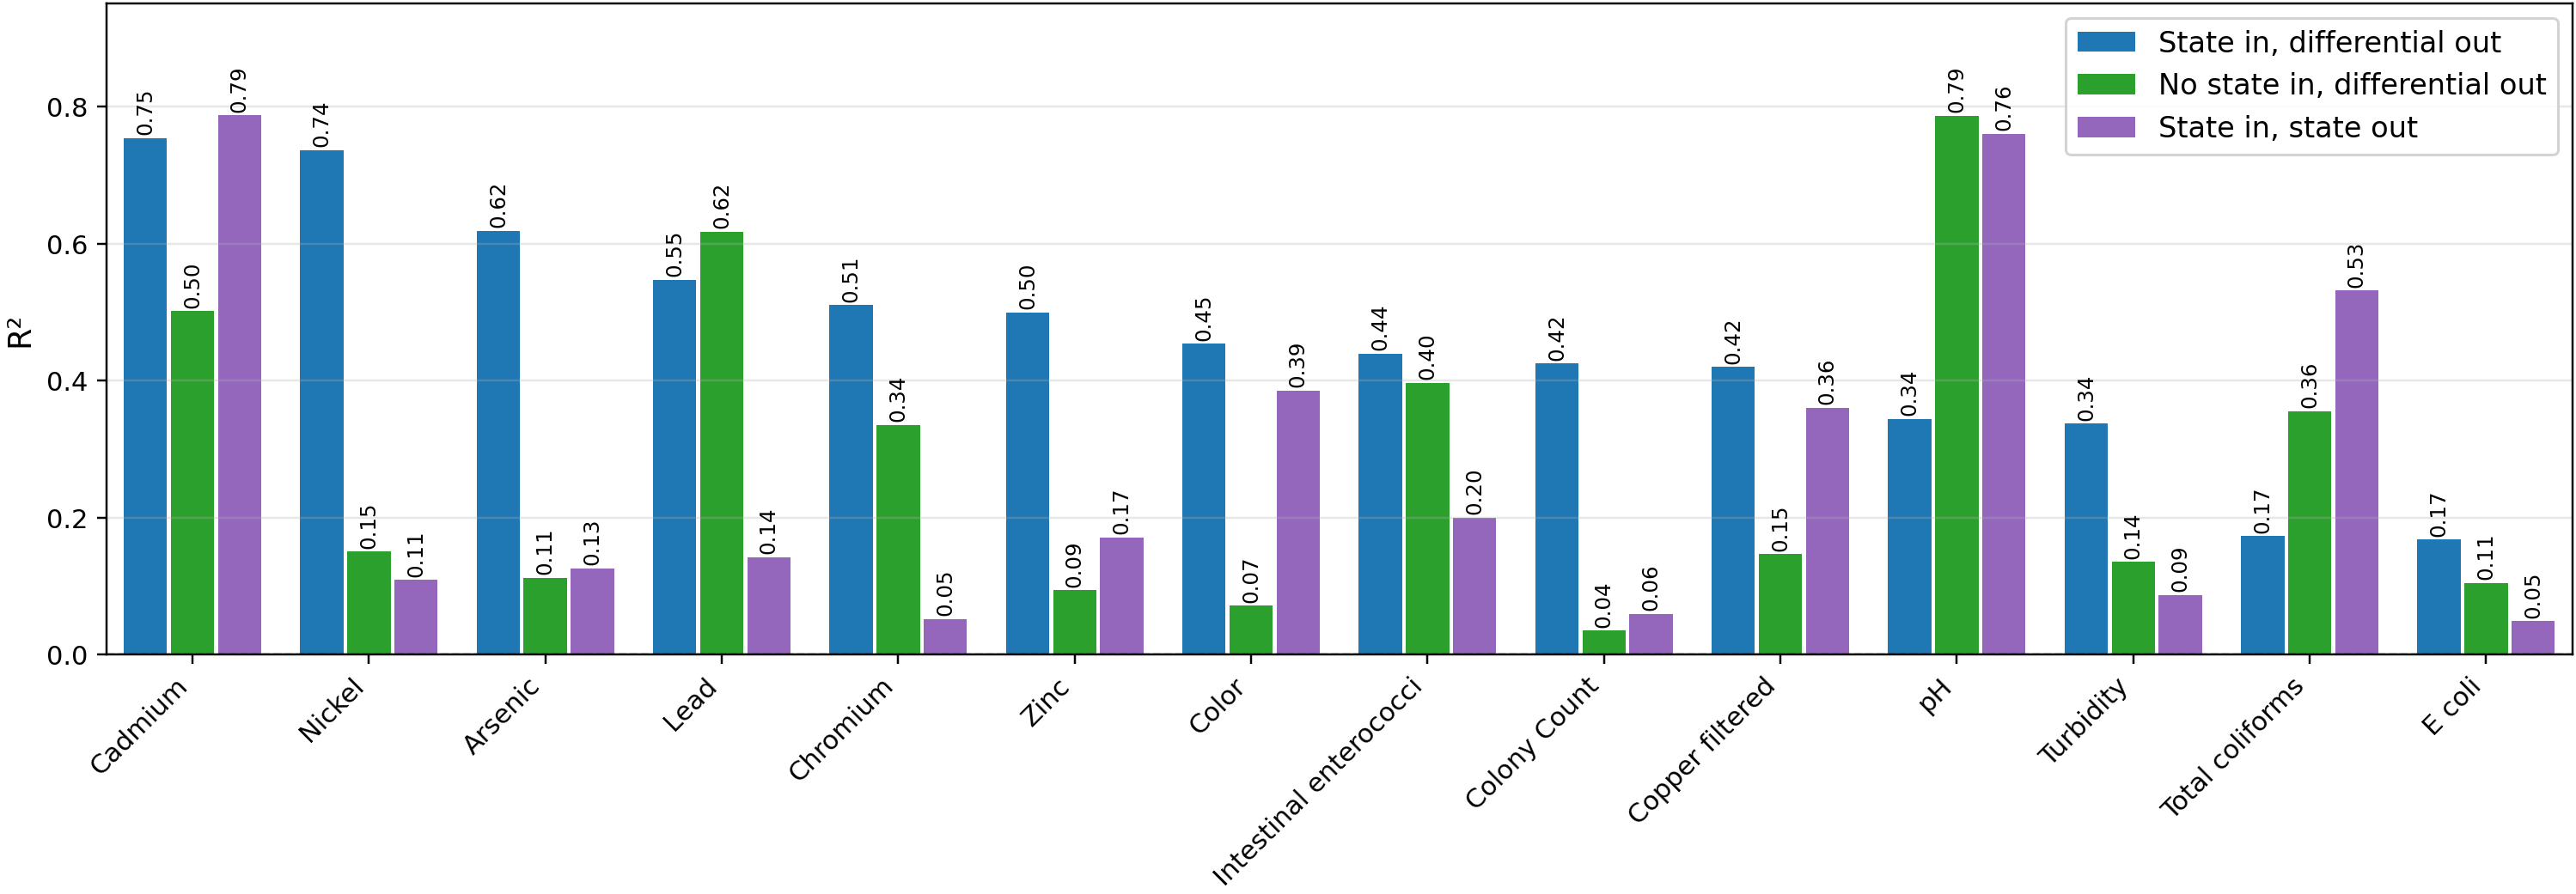
\includegraphics[width=1\linewidth]{figures/r2.png}
    \caption{R\textsuperscript{2} for best ML model.}
    \label{fig:structure}
\end{figure}


\subsection{Feature Selection}
Each target feature has unique sensitivity to predictor features. Aggregating sensitivity across all targets is one method for ranking the relative contribution of each sensor across the study. The estimated Shapley values representing the contribution of each predictor are shown in Fig.~\ref{fig:Shapley}. Per-target Shapley values are z-scored (standardized) to allow direct comparison across targets. The category of predictors consisting of the last measured value of a target, which are only included among predictors for the corresponding target, are shown on the lower pair of axis. For many targets this state estimate for each target is the single most important predictor of the differential in that parameter at the next measurement.

\begin{figure}
    \centering
    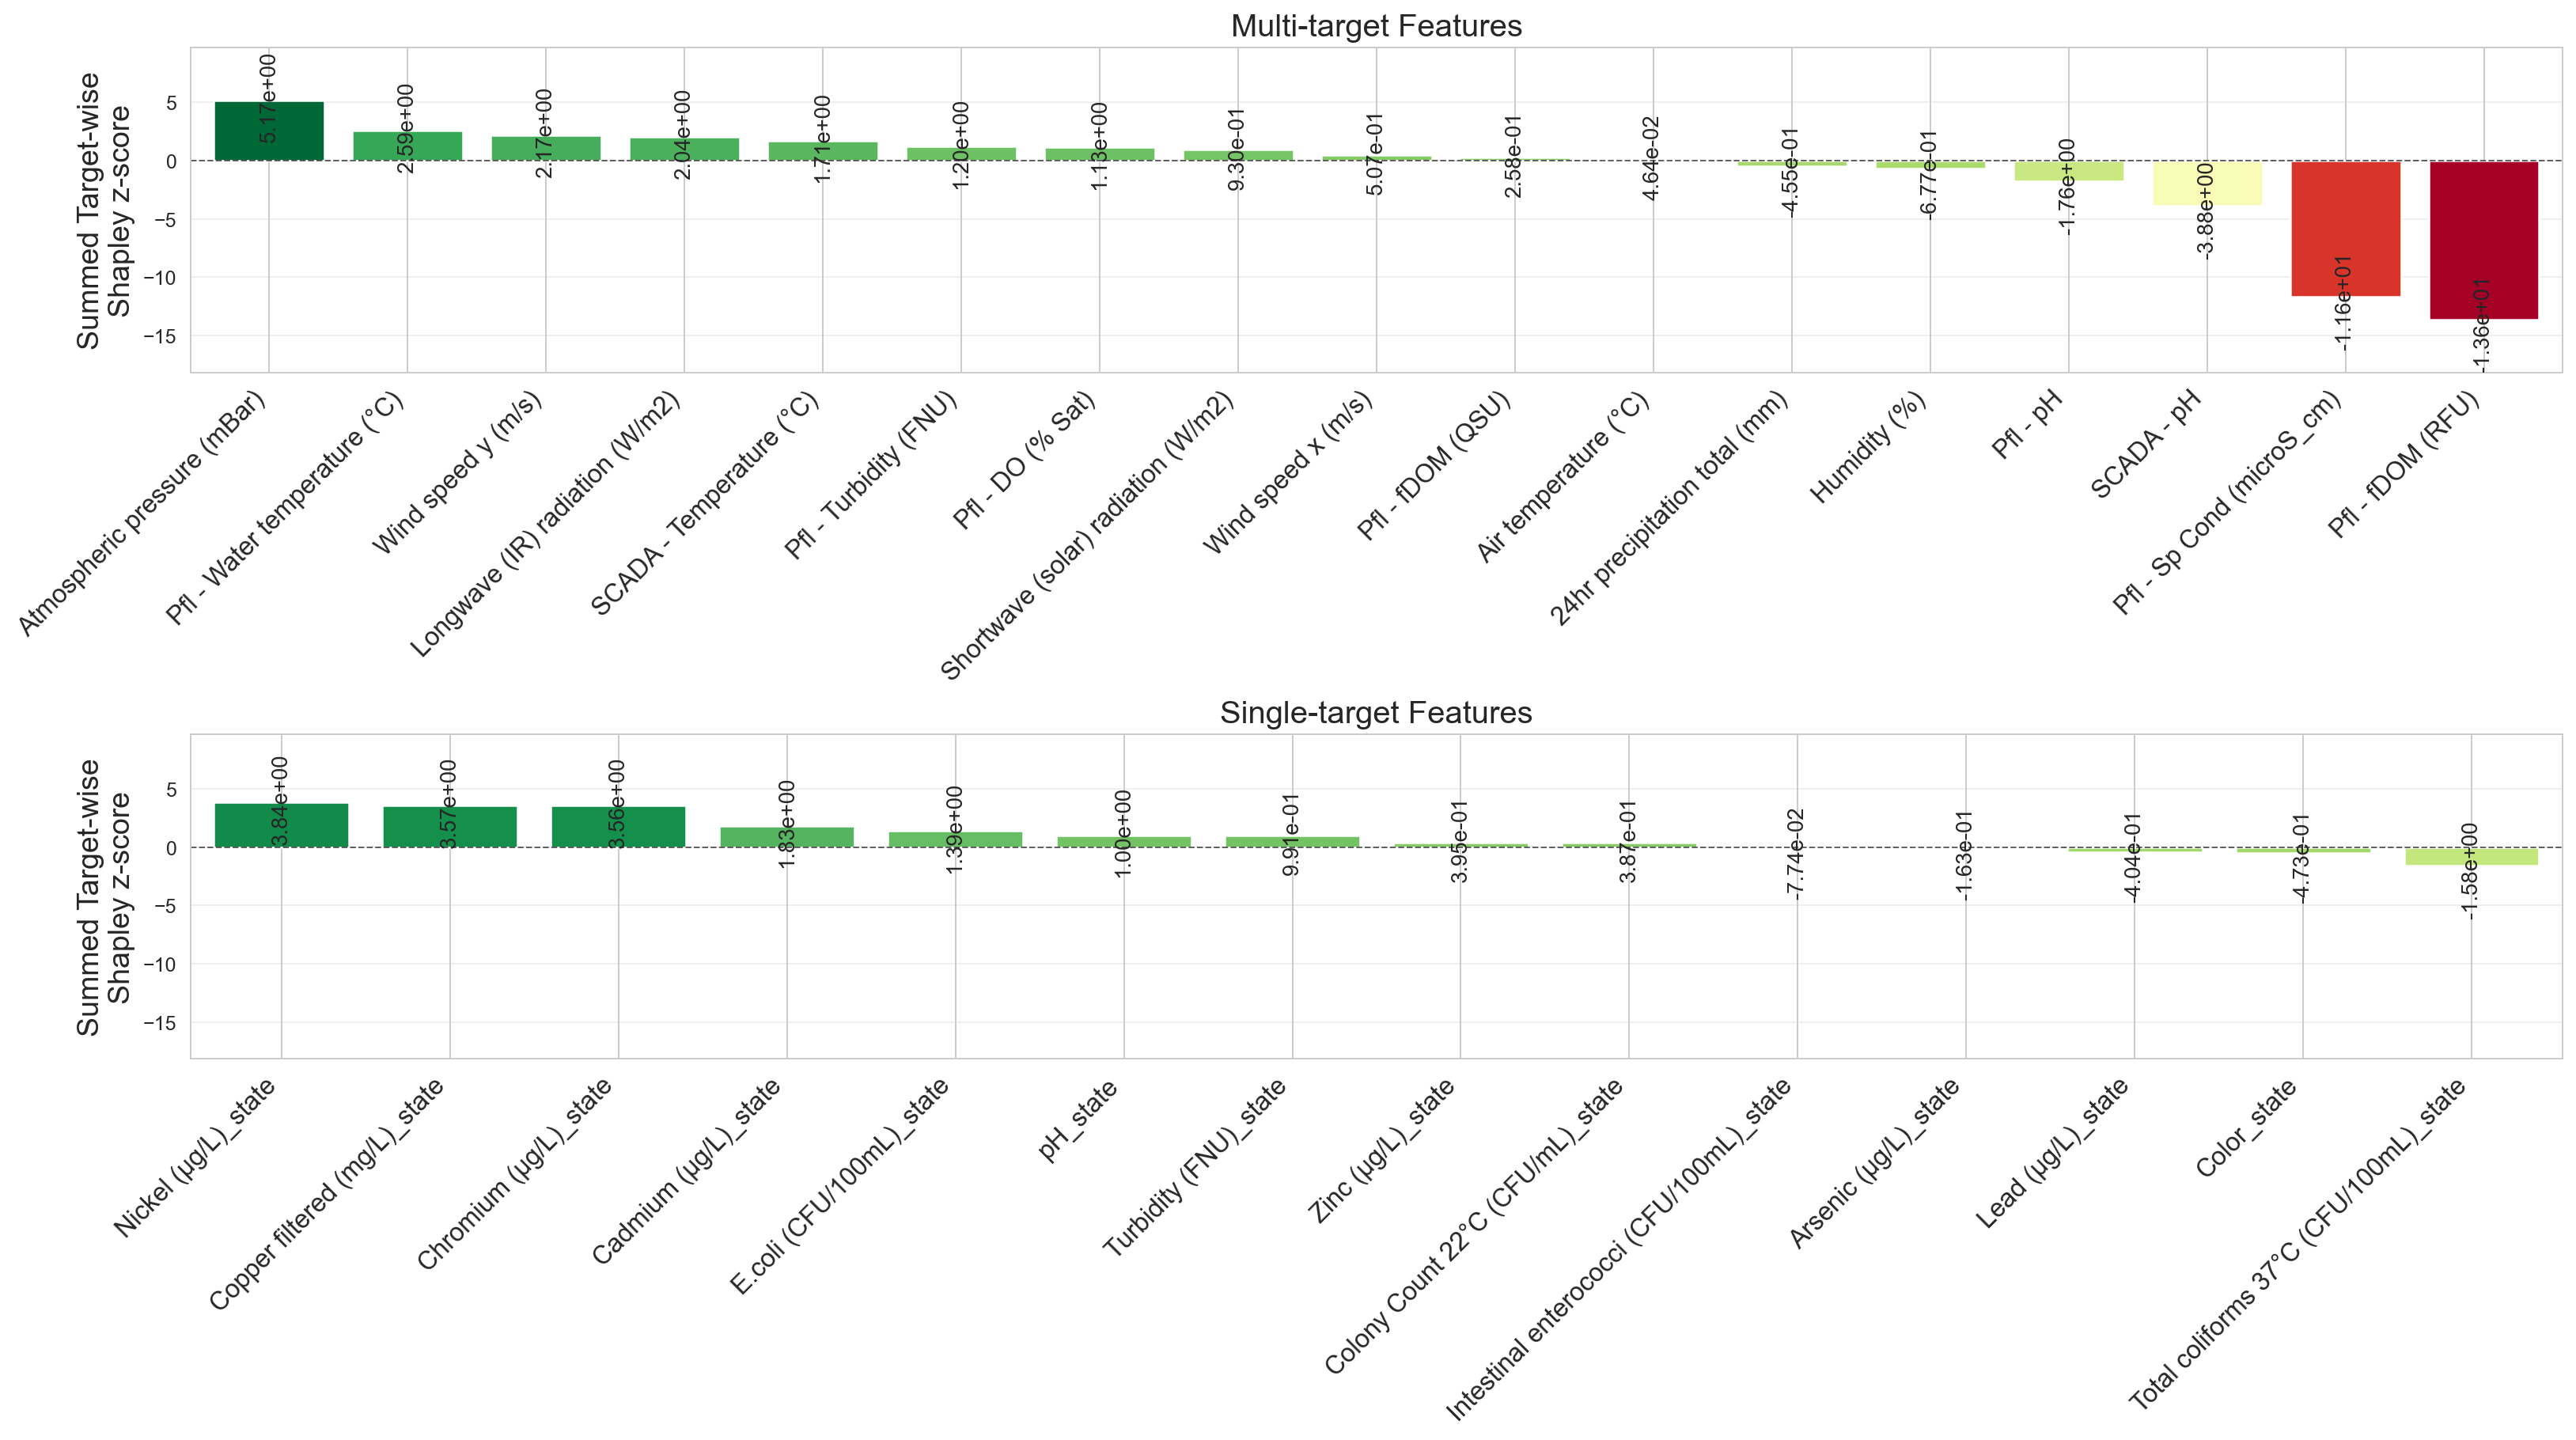
\includegraphics[width=1\linewidth]{figures/multi_target_importance_bars.png}
    \caption{Estimated feature importance aggregated across targets.}
    \label{fig:Shapley}
\end{figure}

However, since these metrics are not weighted by the quality of the predictions by the model, it is also necessary to consider the contribution of sensors by targets. Fig.~\ref{fig:inclusion} presents the features which are included in the best-performing model for each target after feature selection.

\begin{figure}
    \centering
    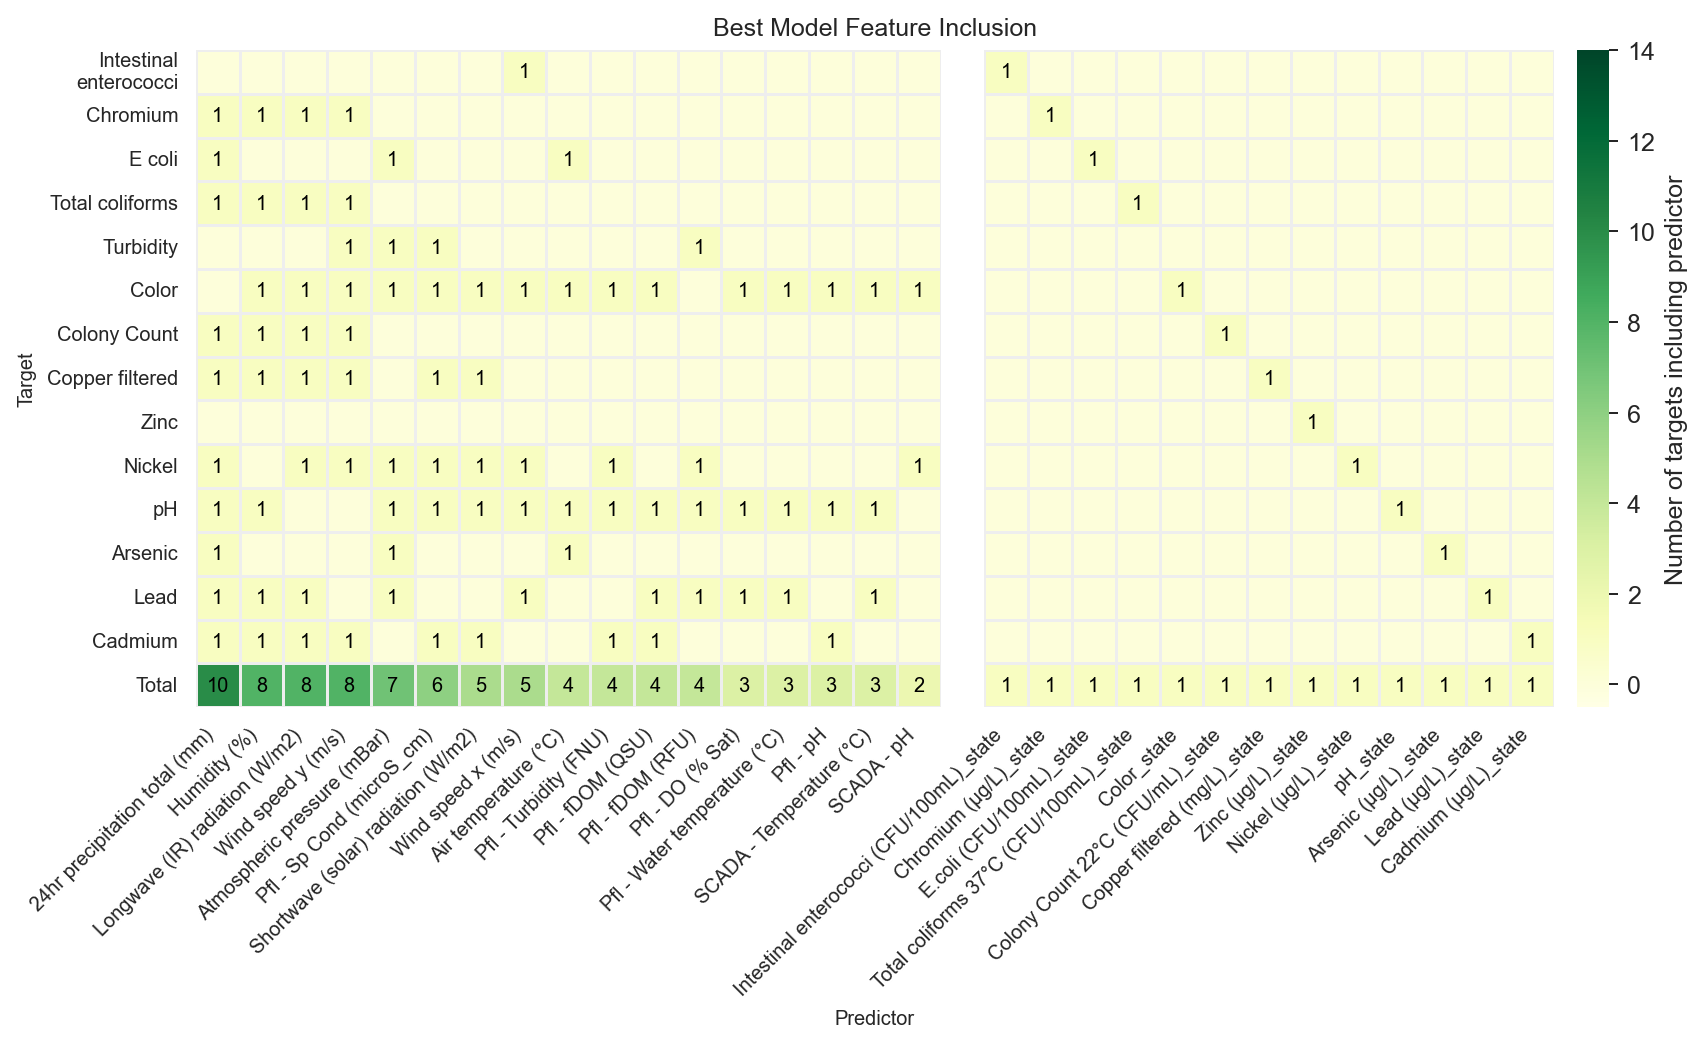
\includegraphics[width=1\linewidth]{figures/multi_target_feature_inclusion_heatmap.png}
    \caption{Predictor feature inclusion for best performing model per target.}
    \label{fig:inclusion}
\end{figure}


\subsection{Hazardous Condition Model Comparisons}
\label{ch:HazardousForecasts}

The performance of the best machine learning model identified within the feature selection search pipeline for predicting target differentials with a one-hour lookahead horizon is summarized in Fig.~\ref{fig:overall}. Key statistics contributing to the evidence score are summarized on the right of the figure, with target sorted by overall Evidence Score.

\begin{figure}
    \centering
    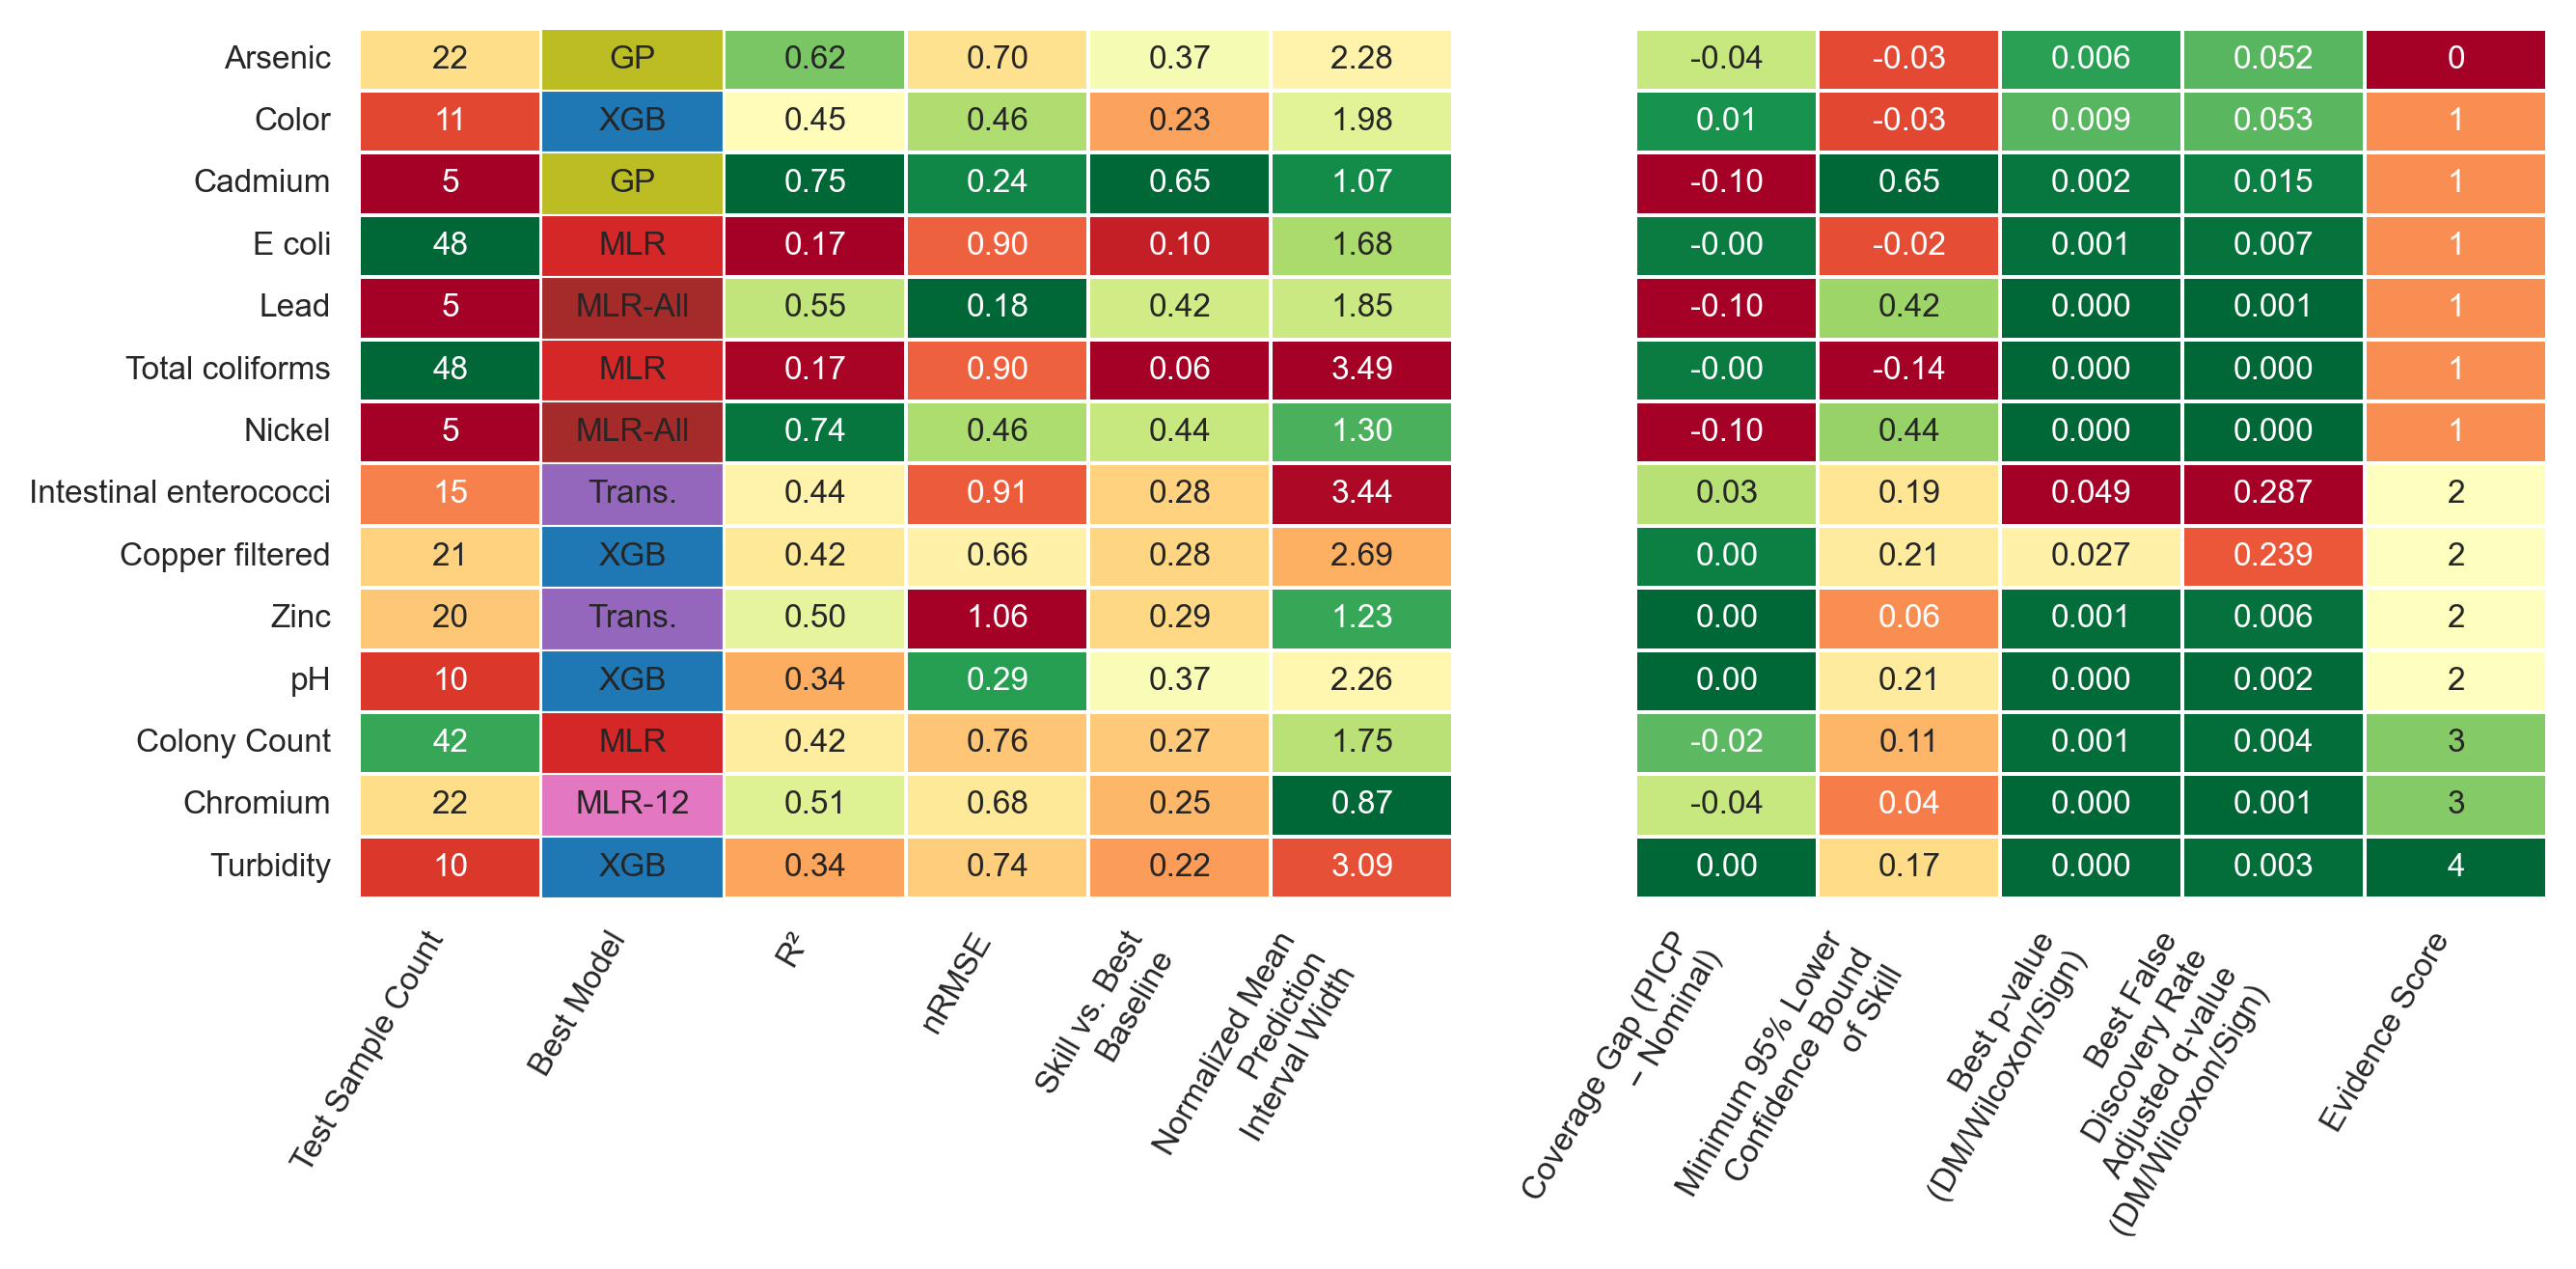
\includegraphics[width=1\linewidth]{figures/summary_model_quality_matrix.png}
    \caption{Best models per target.}
    \label{fig:overall}
\end{figure}

To highlight relative performance by different model architectures, the normalized RMSE of the best-performing iteration of each of the model types for each target are plotted in Fig.~\ref{fig:allmodels}. 

\begin{figure}
    \centering
    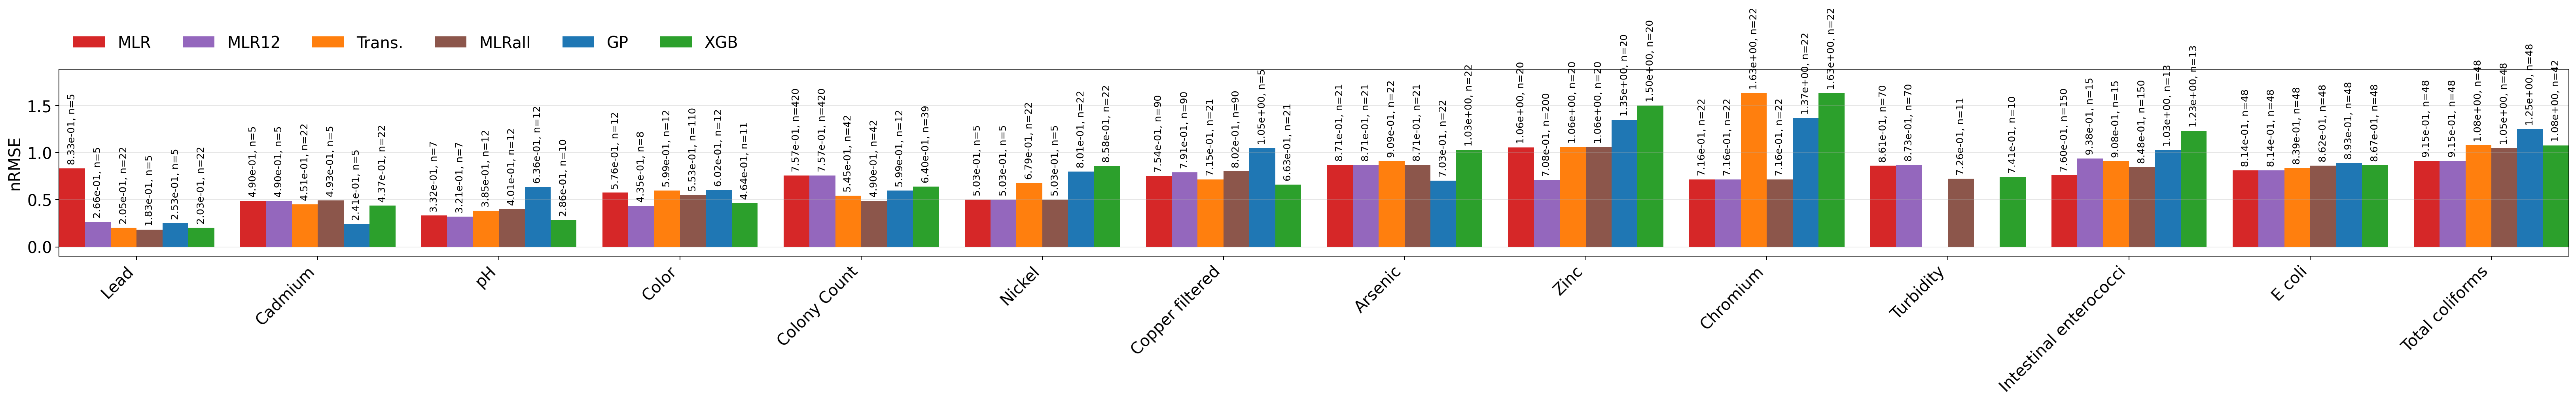
\includegraphics[width=1\linewidth]{figures/ml_comparison_nrmse.png}
    \caption{RMSE normalized by target standard deviation for all model methods.}
    \label{fig:allmodels}
\end{figure}


\subsection{Forecast Horizon Sensitivity}
\label{ch:ForecastHorizon}

Sensitivity of forecast skill to forecast horizon for each of the models are summarized in Fig.~\ref{fig:horizon}, which shows the horizon forecast over which the R\textsuperscript{2} decreases to the greater of the either 0, based on the the average rate of decrease as horizons increase from 1 to 168 hours.    

\begin{figure}
    \centering
    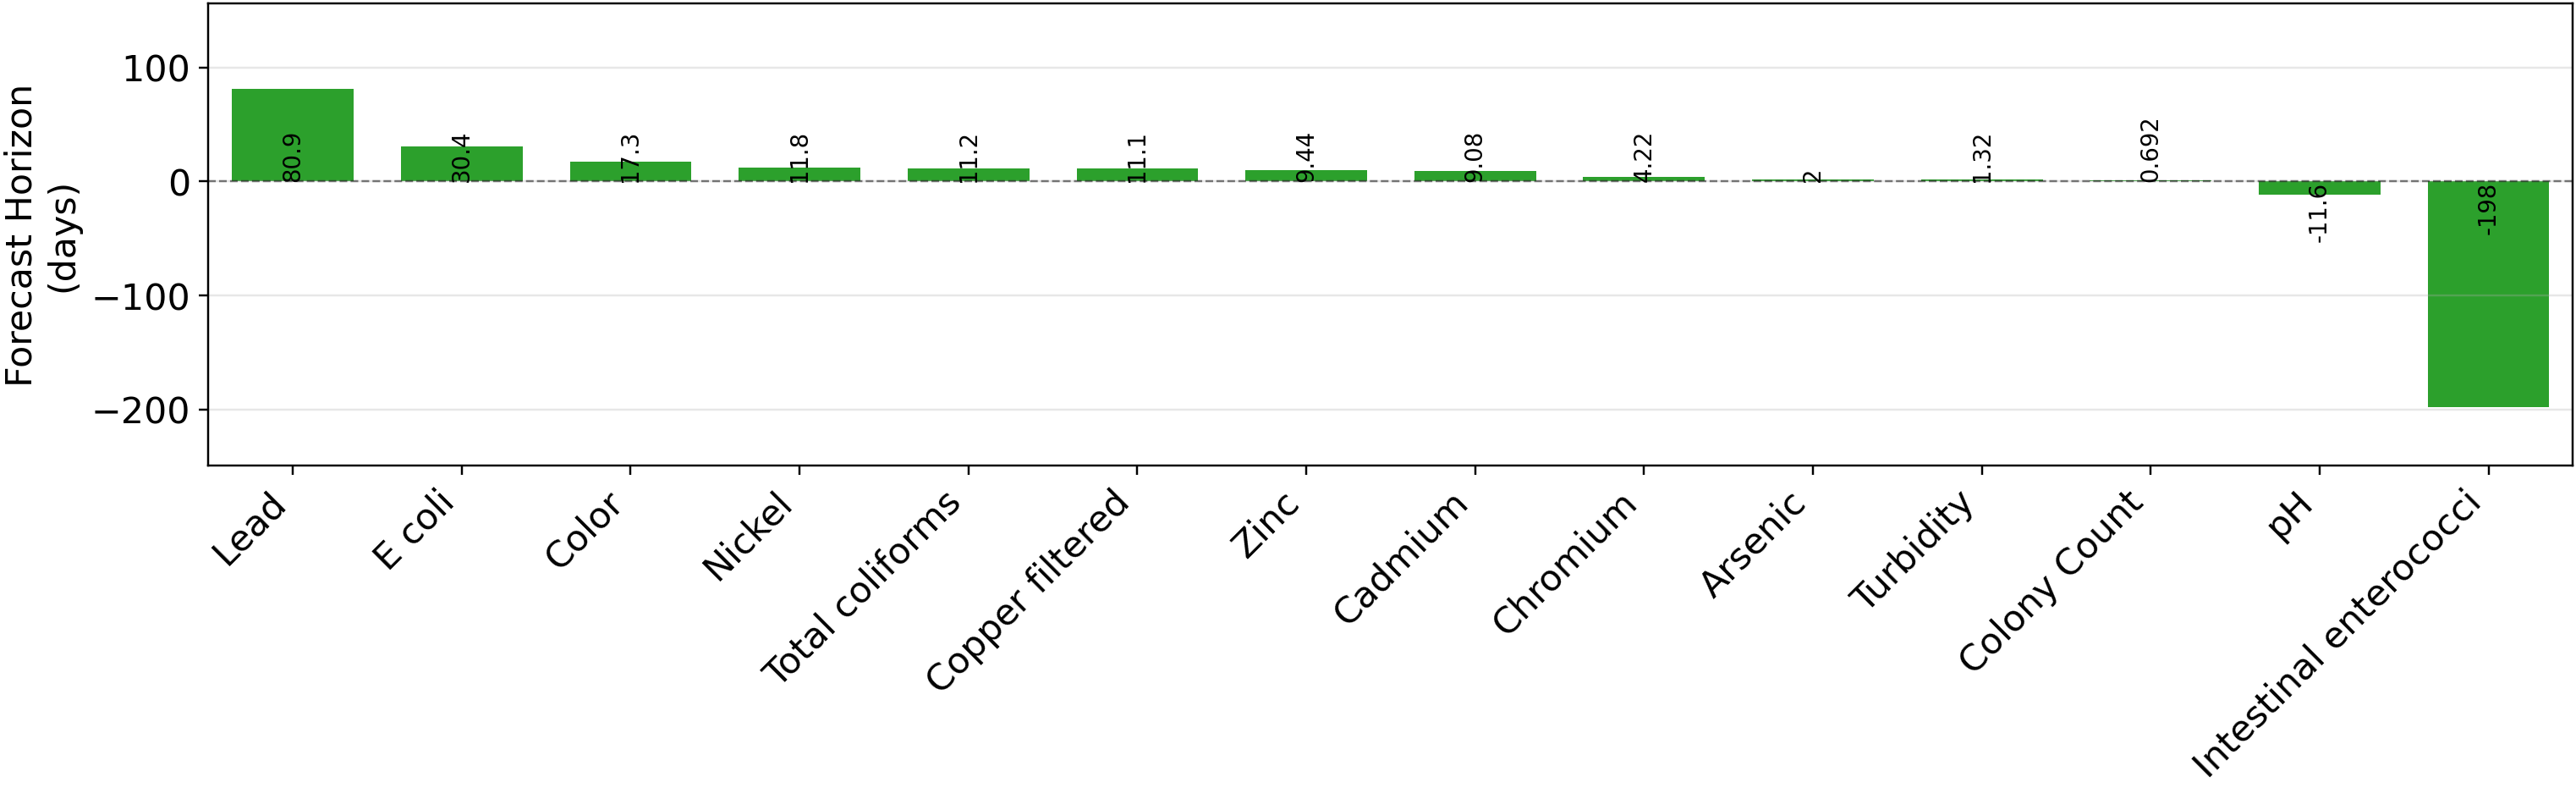
\includegraphics[width=1\linewidth]{figures/lookahead_time_to_baseline_r2.png}
    \caption{Forecast horizon where R\textsuperscript{2} = 0.}
    \label{fig:horizon}
\end{figure}

%%%%%%%%%%%%%%%%%%%%%%%%%%%%%%%%%%%%%%%%%%
\section{Discussion}
\label{ch:Discussion}

Fig.~\ref{fig:structure}, Fig.~\ref{fig:Shapley} and Fig.~\ref{fig:inclusion} all indicate that with the available sample size and features, the machine learning methods evaluated in this study demonstrate the ability to make stable, trustworthy forecasts of the target water quality parameters are significantly enhanced when the last known value of the parameter is included as a predictor. This is expected: none of the indicator water quality parameters measured by sensors are strongly correlated with the target substances at the low concentrations seen in the study. Likewise, the processes which affect concentrations do not depend solely on the weather processes which are represented by the available dataset.

When the sensor dataset is combined with the prior value of the target, two chemical and physical parameter can be reliably forecast with significantly greater skill than baseline methods for all parameters, as shown in Fig.~\ref{fig:overall}.

The differences in performance between diferent model approaches are not large, as highlighted in Fig.~\ref{fig:allmodels}. For six targets, simple multiple linear regression models over aggregated or instantaneous sensor readings outperform more complex models.

The relationship between individual predictor features and targets is complex, with significant variation between targets. In general, the most significant predictor features as measured by either Shapley score or removal sensitivity are Weather features and the prior state. While Surface features can improve forecast skill, a confounding factor in this analysis is the inconsistent coverage between features. The Surface features have lower coverage, resulting in either fewer valid samples or less data per sample compared to predictor combinations which exclude features of the Surface set. The coverage is biased: the majority of the missing coverage occurs during winter months due to practical limits on sensor operation. With the available data, if samples are restricted to periods with full coverage by Surface features while preserving temporal split between training and test sets, the result is extremely small sets with unstable results and underpowered statistical tests.


\begin{itemize}
    \item Information about the initial value of the target allows machine learning models to provide more accurate forecasts than common baseline methods by targeting the difference from the previous value.
    \item In particular, the XGBRegressor method provides the most accurate forecasts for all available targets with sufficient sample size.
    \item For all models which provided acceptably accurate forecasts, the accuracy is relatively insensitive to forecast horizon over the range of horizons evaluated, which is up to one week. 
    \item Although the sensitivity to predictor features varies significantly between targets
\end{itemize}



The strong performance of the XGBoost-based models across diverse targets and features sets confirms the suitability of this machine learning method for regression 

While these results demonstrate the feasibility of using data-driven methods to forecast water quality, implementing an operational, continuously updated forecasting system to provide consistent decision support for water quality management would raise additional practical challenges were are not addressed within the scope of this paper. 

% Emphasize implications for other applications, i.e. thesis goal of digital twins of the coastal environment

% Authors should discuss the results and how they can be interpreted from the perspective of previous studies and of the working hypotheses. The findings and their implications should be discussed in the broadest context possible. Future research directions may also be highlighted.

%%%%%%%%%%%%%%%%%%%%%%%%%%%%%%%%%%%%%%%%%%
% \section{Conclusions}

% This section is not mandatory, but can be added to the manuscript if the discussion is unusually long or complex.
%%%%%%%%%%%%%%%%%%%%%%%%%%%%%%%%%%%%%%%%%%
\vspace{6pt} 

%%%%%%%%%%%%%%%%%%%%%%%%%%%%%%%%%%%%%%%%%%
%% optional
% \supplementary{The following supporting information can be downloaded at:  \linksupplementary{s1}, Figure S1: title; Table S1: title; Video S1: title.}

%%%%%%%%%%%%%%%%%%%%%%%%%%%%%%%%%%%%%%%%%%
\authorcontributions{Conceptualization, X.X., Y.Y. and Z.Z.; methodology, ; software, ; validation, ; formal analysis, ; investigation, ; resources, ; data curation, ; writing---original draft preparation, ; writing---review and editing, ; visualization, ; supervision, ; project administration, ; funding acquisition, R.S. All authors have read and agreed to the published version of the manuscript.}

\funding{This research was funded by Møre og Romsdal Fylkeskommune grant number 100735100. The APC was funded by NTNU.}

\dataavailability{The original data presented in the study are openly available in GitHub at \url{https://github.com/russellprimeau/WQRegressors}.} 

\acknowledgments{In this section you can acknowledge any support given which is not covered by the author contribution or funding sections. This may include administrative and technical support, or donations in kind (e.g., materials used for experiments). Where GenAI has been used for purposes such as generating text, data, or graphics, or for study design, data collection, analysis, or interpretation of data, please add “During the preparation of this manuscript/study, the author(s) used [tool name, version information] for the purposes of [description of use]. The authors have reviewed and edited the output and take full responsibility for the content of this publication.”}

\conflictsofinterest{The authors declare no conflicts of interest.} 

\appendixtitles{no} % Leave argument "no" if all appendix headings stay EMPTY (then no dot is printed after "Appendix A"). If the appendix sections contain a heading then change the argument to "yes".
\appendixstart
\appendix
\section[\appendixname~\thesection]{}
\subsection[\appendixname~\thesubsection]{}
The appendix is an optional section that can contain details and data supplemental to the main text---for example, explanations of experimental details that would disrupt the flow of the main text but nonetheless remain crucial to understanding and reproducing the research shown; figures of replicates for experiments of which representative data are shown in the main text can be added here if brief, or as Supplementary Data. Mathematical proofs of results not central to the paper can be added as an appendix.

\begin{table}[H] 
\caption{This is a table caption.\label{tab5}}
%\newcolumntype{C}{>{\centering\arraybackslash}X}
\begin{tabularx}{\textwidth}{CCC}
\toprule
\textbf{Title 1}	& \textbf{Title 2}	& \textbf{Title 3}\\
\midrule
Entry 1		& Data			& Data\\
Entry 2		& Data			& Data\\
\bottomrule
\end{tabularx}
\end{table}

\section[\appendixname~\thesection]{}
All appendix sections must be cited in the main text. In the appendices, Figures, Tables, etc. should be labeled, starting with ``A''---e.g., Figure A1, Figure A2, etc.

%%%%%%%%%%%%%%%%%%%%%%%%%%%%%%%%%%%%%%%%%%
%\isPreprints{}{% This command is only used for ``preprints''.
\begin{adjustwidth}{-\extralength}{0cm}

\reftitle{References}

\bibliography{sources}

%%%%%%%%%%%%%%%%%%%%%%%%%%%%%%%%%%%%%%%%%%
\PublishersNote{}
%\isPreprints{}{% This command is only used for ``preprints''.
\end{adjustwidth}
%} % If the paper is ``preprints'', please uncomment this parenthesis.
\end{document}

